\chapter{مدل پیشنهادی و کار‌های صورت گرفته}
در این فصل به تبیین ساز و کار ارائه شده پرداخته می‌شود. در ابتدای فصل، دادگان انتخاب شده برای آزمایش‌های صورت گرفته روی مدل‌های محاسباتی معرفی می‌شود. در بخش بعدی، جزئیات و پارامترهای شبکه‌ی سلسله مراتبی که در فصل پیش معرفی شد بیان می‌شود. پس از آن مکانیسم‌های برقراری اتصالات سیناپسی در ماشین‌های حالت مایع مورد بررسی قرار می‌گیرد. این بخش همچنین مدل نورونی و مدل سیناپسی را به همراه نحوه‌ی شکل‌پذیری سیناپسی بیان می‌کند. در نهایت با معرفی معیار میزان تفکیک‌پذیری و همچنین به کار بردن دو طبقه‌بند، نحوه‌ی عملکرد ماشین حالت مایع تحت پارامترهای مختلف عرضه می‌گردد.
\section{دادگان استفاده شده}
جهت ارزیابی کارایی معماری عرضه شده از دو مجموعه‌ی داده‌ی \lr{CALTECH}\footnote{قابل بارگذاری از \lr{http://www.vision.caltech.edu/}} با عناوین \lr{Motorcycles 2001} و \lr{Faces 1999} استفاده شده است. هر مجموعه‌ی داده به دو مجموعه‌ی آموزشی (جهت استفاده در گام یادگیری شبکه) و آزمون (جهت ارزیابی شبکه در گام آزمون) افراز شده است. ابعاد تصاویر با هم فرق داشته و از این جهت با ثابت گرفتن ارتفاع تصویر روی ۳۰۰ پیکسل، با حفظ نسبت ابعاد\footnote{\lr{Aspect ratio}}، مقیاس‌بندی مجدد شده‌اند. علاوه بر آن، از آنجایی که تحقیق جاری بر روی نقش رنگ‌ها در بازشناسی تمرکز ندارد، تصاویر به طیف رنگ خاکستری تبدیل شده‌اند. نمونه‌ی تصاویر استفاده شده را می‌توان در شکل \ref{fig:sample_input} مشاهده نمود. به طور خلاصه برای ارزیابی کارایی مدل‌ها، در گام آموزش و آزمون به ترتیب ۱۵۰ و ۲۸۵ نمونه استفاده شده است. لازم به ذکر است که از ۱۵۰ تصویر به کار رفته، صرفا تعداد ۱۰۰ تصویر جهت آموزش شبکه‌ی سلسله مراتبی استفاده می‌شود که به موجب آن توانایی تعمیم‌پذیری بیشتری طبق آزمایش‌ها حاصل شده است.


\begin{table}[]
\centering
\caption{تعداد نمونه‌های ورودی}
\label{my-label}
\begin{tabular}{|r|c|l|}
\hline
\multicolumn{1}{|c|}{کلاس} & بخش & \multicolumn{1}{c|}{تعداد نمونه} \\ \hline
\multirow{2}{*}{صورت}       & Train    & 218                                \\ \cline{2-3}  & Test     & 217                                \\ \hline
\multirow{2}{*}{موتورسیکلت} & Train    & 400                                \\ \cline{2-3} & Test     & 400                                \\ \hline
\end{tabular}
\end{table}

\begin{figure}
\centering
{\footnotesize
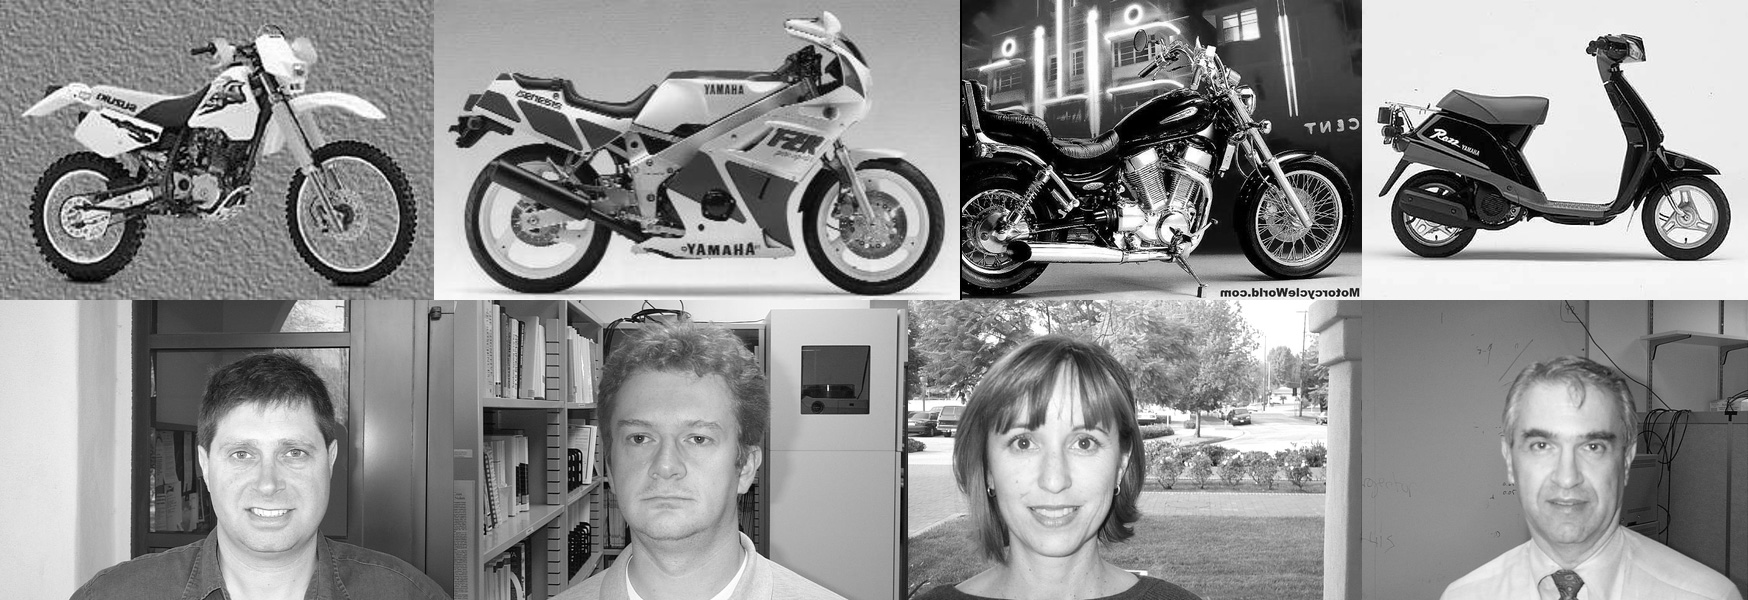
\includegraphics[height=5.5cm]{sample_input}
\caption[نمونه تصاویر ورودی]{نمونه تصاویر ورودی (متشکل از تصاویر موتورسیکلت و صورت انسان) که برای آموزش و ارزیابی کارایی استفاده شده اند.}
\label{fig:sample_input}
}
\end{figure}

در ادامه به دو مولفه‌ی اصلی تشکیل‌دهنده‌ی مدل ارائه شده می‌پردازیم و به تفصیل هر کدام را با جزییات معرفی خواهیم کرد.

\section{شبکه سلسله مراتبی}
دادگان ورودی در ابتدا وارد شبکه‌ی سلسله مراتبی می‌شوند. مدل سلسله مراتبی از سلول‌های ساده و پیچیده تشکیل می‌شوند. طی عملیات سلول‌های ساده، گزینندگی مناسب نورون شکل می‌پذیرد در حالی که در نتیجه‌ی عملیات سلول‌های پیچیده، مدل نسبت به مقیاس و موقعیت مقاوم می‌شود. 

\subsection{لایه‌های شبکه‌ی سلسله مراتبی}
چهار لایه نورون در این مدل به شرح ذیل هستند:

\begin{itemize}
\item
\textbf{سلول‌های \lr{S1}}، با اعمال یک همگشت یا پیچش\footnote{\lr{Convolution}} روی تصویر ورودی، لبه‌ها را شناسایی می‌کنند. ما برای این لایه، از ساز و کار نورونی (که پیشتر نحوه‌ی تشکیل و عملکردشان تبیین شده است) استفاده نکرده و صرفا از اعمال فیلتر‌های $5\times5$ گابور\footnote{\lr{Gabor}} بدست می‌آید که طول موج ۵، عرض موثر ۲ و چهار جهت ارجح ($\pi/8$، $\pi/4+\pi/8$، $\pi/2+\pi/8$ و $3\pi/4+\pi/8$) دارند. فیلتر‌ها روی پنج مقیاس از تصویر ورودی، یعنی $100\%$ (تصویر اصلی)، $70\%$، $50\%$، $36\%$ و $25\%$، اعمال می‌گردند. پس با در نظر گرفتن پنج مقیاس و چهار زاویه‌ی جهت‌گیری، شبکه شامل ۲۰ نقشه‌ی \lr{S1} است. سلول‌های \lr{S1} ضربه‌هایی با تاخیر متناسب با معکوس شدت پاسخ فیلتر تولید می‌کنند. به عبارت دیگر، هر چه محرک با جهت‌گیری نورون انطباق بیشتری داشته باشد، سریعتر ضربه پاسخ آن تولید می‌شود. فعالیت نورونی همچنین در این لایه محدود می‌شود و در هر مقیاس و موقعیت تنها ضربه‌ی بهترین جهت مورد انطباق انتقال می‌یابد. 

\item
\textbf{سلول‌های \lr{C1}} اولین ضربه‌های دریافت شده از سلول‌های \lr{S1} قرار گرفته در یک میدان تاثیر مربعی $7\times7$ از یک نقشه‌ی \lr{S1} را پردازش می‌کنند. هر نقشه‌ی \lr{S1} متناظر با یک جهت و یک مقیاس است. دو سلول \lr{C1} که در یک نقشه‌ی \lr{C1} کنار هم قرار گرفته‌اند متناظر با دو میدان تاثیر مربعی $7\times7$ از سلول‌های \lr{S1} هستند که به اندازه‌ی ۶ واحدِ \lr{S1} از هم فاصله داشته و به اندازه‌ی یک نورونِ \lr{S1} همپوشانی دارند. پس با در نظر نگرفتن گوشه‌ها، سلول‌های \lr{C1} چیزی در حدود $6\times6=36$ بار کمتر از سلول‌های \lr{S1} هستند.
عملگر ادغام بیشینه که نسبت به تغییر موقعیت، ناوردایی ایجاد می‌کند از لحاظ زیستی قابل پذیرش است\cite{riesenhuber1999hierarchical}. 
علاوه بر زیرنمونه گرفتن در این لایه، مکانیسم منکوب جانبی\footnote{\lr{Lateral inhibition}} به کار برده شده است که در نتیجه‌ی آن اگر یک ناحیه به وضوح برای یک جهت غالب باشد، سلول‌های دیگر را با افزایش تاخیر آنها مهار کرده و در نتیجه‌ی STDP تقویت بیشتری می‌یابد. مکانیسم مهار جانبی به این نحو است که به موجب یک ضربه‌ی \lr{C1}، تاخیر همسایگانش در همسایگی $11\times11$ از نقشه با همان مقیاس و جهت افزایش می‌یابد. 

\item
\textbf{سلول‌های \lr{S2}} از لحاظ پیچیدگی ویژگی‌های بصری در سطح بالاتری قرار می‌گیرند. در تحقیق جاری ما تنها از چهار عدد سلول نمونه‌ی \lr{S2}، به جهت تمرکز و تبیین بهتر عملکرد ماشین حالت مایع که در بخش بعد توضیح داده خواهد شد استفاده کرده‌ایم. در واقع به ازای هر سلول نمونه، پنج نورون با پنج نقشه (به ازای هر مقیاس) وجود دارد که با مکانیسم اشتراک وزنی\footnote{\lr{Weight sharing}} کار می‌کنند. در هر نقشه، سلول \lr{S2} تنها می‌تواند ضربه‌های چهار نقشه‌ی \lr{C1} در جهت‌های مختلف متناظر با مقیاس مورد پردازش را تجمیع کند. میدان تاثیر به اندازه‌ی $16\times16$ سلول \lr{C1} و $96\times96$ سلول \lr{S1} خواهد بود. همچنین اتصالات سیناپسی از \lr{C1} به \lr{S2} با به کارگیری STDP میزان‌سازی می‌شوند. 

لازم به ذکر است که فعالیت نورونی نیز محدود می‌شود. با استفاده از یک مکانیسم \lr{k-winner-take-all}، حداکثر دو نورون به ازای هر مقیاس پردازشی می‌توانند آتش کنند. این مکانیسم که تنها در گام یادگیری استفاده می‌گردد به یادگیری الگوها در اندازه‌ها و مقیاس‌های مختلف کمک می‌کند. بدون این مکانیسم، گرایش به یادگیری الگو‌های کوچکتر (مقیاس‌های بزرگتر) وجود داشته و بخاطر بزرگتر بودن نقشه‌های متناظر، احتمال ضربه با وزن تصادفی در ابتدا‌ی فرآیند STDP بالا می‌بود. 

\item
\textbf{سلول‌های \lr{C2}} برای هر نمونه بیشترین پاسخ (یعنی اولین ضربه) از سلول‌های \lr{S2} متناظر را در همه‌ی موقعیت‌ها و مقیاس‌ها گرفته و در نتیجه چهار نورون با ناوردایی نسبت به موقعیت و مقیاس خواهیم داشت.
\end{itemize}
\subsection{مدل STDP برای شبکه‌ی سلسله مراتبی}

مدل STDP از یک قاعده‌ی ساده بهره می‌برد:

\begin{equation} 
\left\{\begin{matrix}
\Delta w_{ij} = a^+w_{ij}(1-w_{ij}) & if \; \; \; t_j-t_i > 0 \\ 
\Delta w_{ij} = a^-w_{ij}(1-w_{ij}) & if \; \; \; t_j-t_i \leq  0
\end{matrix}\right.
\end{equation} 
که $i$ و $j$ به ترتیب  نمایانگر نورون‌های پیش و پس‌سیناپسی هستند که زمان ضربه‌ی آنها با  $t_i$ و $t_j$ نمایش داده شده است. $\Delta w_{ij}$ تغییر وزن سیناپس متصل کننده‌ی $i$ به $j$ را نشان می‌دهد و $a^+$ و $a^-$ دو پارامتری هستند که میزان تغییرات را تعیین می‌کنند. همانطور که از معادله‌ی بالا بر می‌آید، تغییرات وزنی بر میزان $t_i-t_j$ وابسته نبوده بلکه صرفا به علامت آن که نشاندهنده‌ی ترتیب دو ضربه نسبت به یکدیگر است وابسته می‌باشند. مورد دیگر این است که پنجره‌ی زمانی برای STDP نامحدود در نظر گرفته شده است. 

\begin{figure}
\centering
{\footnotesize
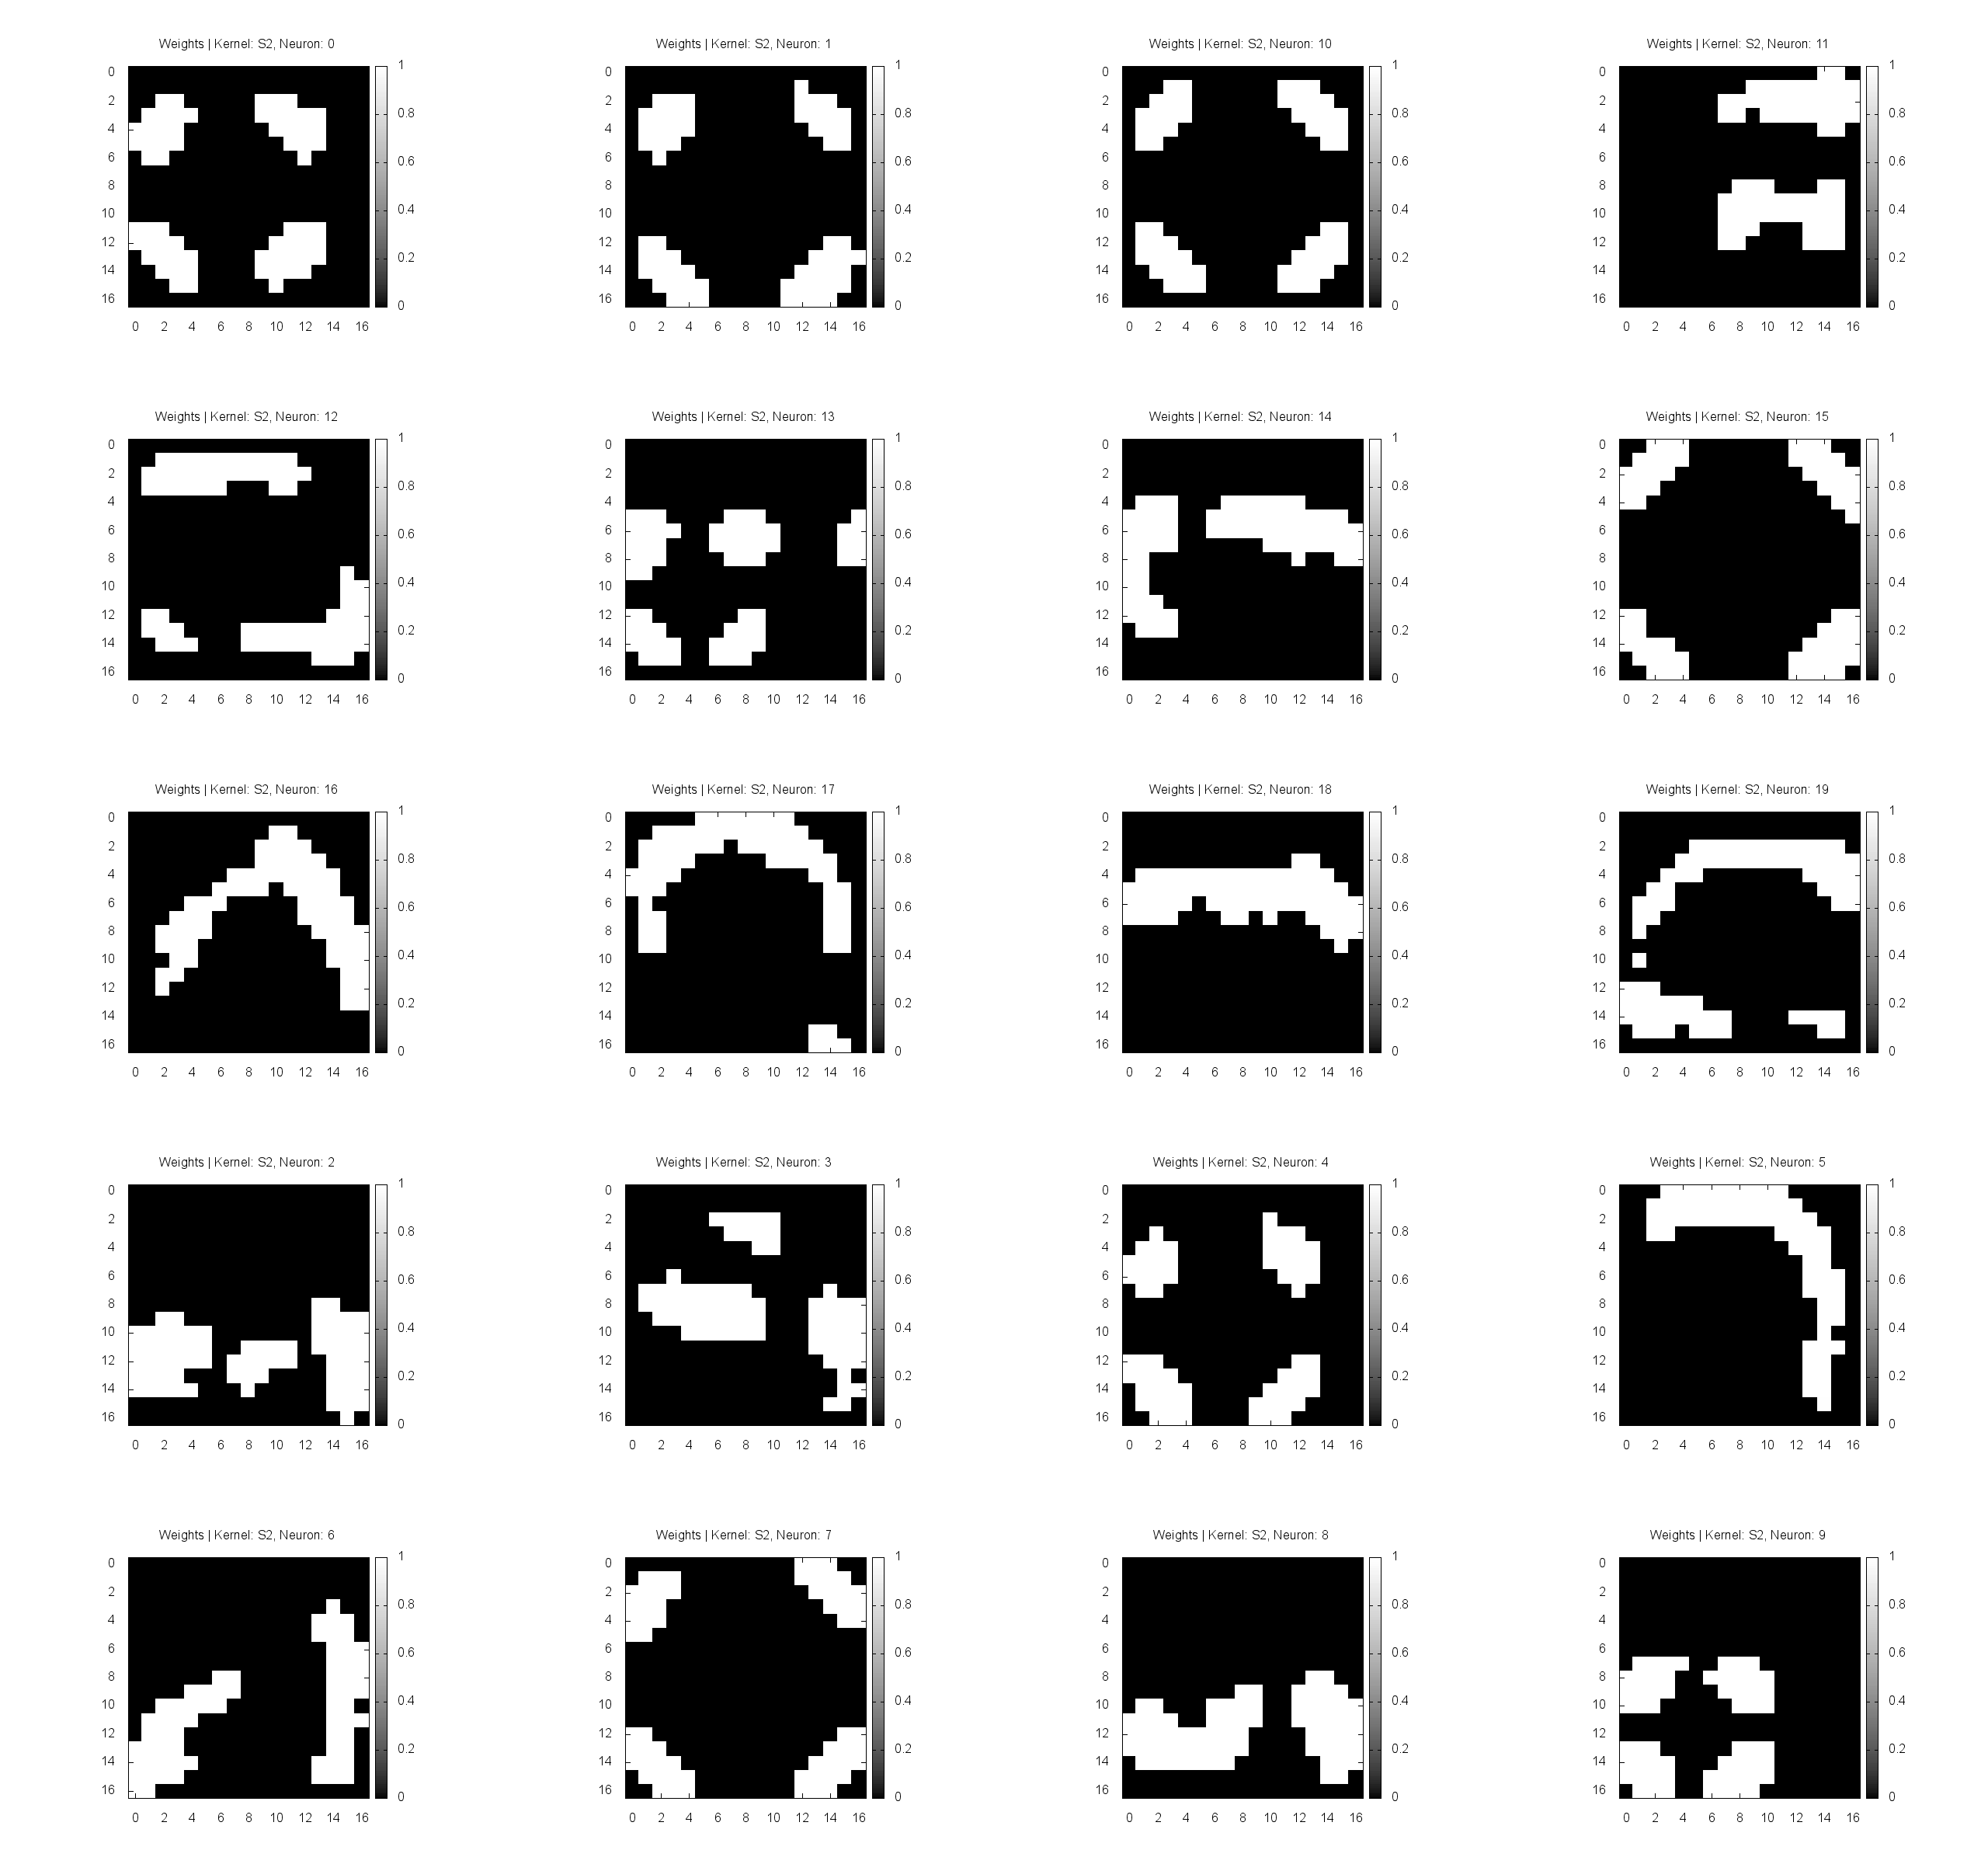
\includegraphics[height=13.5cm]{hierarchi_RFs}
\caption{نمونه میدان‌های تاثیر شبکه‌ی سلسله مراتبی}
\label{fig:hierarchi_RFs}
}
\end{figure}

\subsection{مدل نورونی و سیناپسی}
مدل نورونی مورد استفاده برای سلول‌های \lr{S2} در مدل سلسله مراتبی از نوع تجمیع و آتش\footnote{\lr{Integrate-and-Fire}} (\lr{IF}) است. این نورون‌ها نیازی به نشتی\footnote{\lr{Leakage}} ندارند. در مغز با استفاده از نشتی، از تداخل موج ضربه‌های پشت سر هم جلوگیری می‌شود که در مدل سلسله‌مراتبی نیاز به آن نیست زیرا پیش از ارائه‌ی تصویر هر محرک ورودی، همه‌ی پتانسیل‌ها مقداردهی مجدد می‌شوند. مدل سیناپسی نیز از نوع مبتنی بر جریان\footnote{\lr{Current Based}}(\lr{CUBA}) می‌باشد به این معنی که ساده‌سازی شده و خاصیت خازنی ندارد.

\subsection{پارامترها و عملکرد شبکه‌ی سلسله مراتبی}

\begin{table}[]
\centering
\caption{پارامترهای شبکه‌ی سلسله مراتبی و مقادیر انتخاب شده}
\label{masq_param_tables}
\begin{tabular}{|l|c|r|}
\hline
\multicolumn{1}{|c|}{پارامتر} & مقدار     & \multicolumn{1}{c|}{توضیحات} \\ \hline
GaborRF             & 5       & عرض و طول میدان تاثیر سلول‌های \lr{S1}  \\ \hline
GaborCRF            & 7       &   عرض و طول میدان تاثیر سلول‌های \lr{C1}    \\ \hline
%GaborDiv            & 4       &        \\ \hline
C1InhibRFsize       & 5       &   اندازه‌ی همسایگی در مهار جانبی    \\ \hline
C1InhibPercentClose & $0.15$    &    حداکثر میزان مهار جانبی (برای نزدیکترین همسایگان)   \\ \hline
C1InhibPercentFar   & $0.05$    &   حداقل میزان مهار جانبی (برای دورترین همسایگان)    \\ \hline
Threshold           & $30$      &   آستانه‌ی آتش سلول‌های ساده    \\ \hline
meanWeight          & $0.8$     &   میانگین توزیع تصادفی نرمال برای وزن‌های سیناپسی    \\ \hline
stdDevWeight        &  $0.05$   &    انحراف معیار توزیع تصادفی نرمال برای وزن‌های سیناپسی   \\ \hline
SRF                 & 17      &   عرض و طول میدان تاثیر سلول‌های \lr{S2}    \\ \hline
CRF                 & 3       &    عرض و طول میدان تاثیر سلول‌های \lr{C2}   \\ \hline
CSTRIDE             & 2       &   میزان پرش از همسایگی برای محاسبه‌ی ادغام بیشینه    \\ \hline
kWTA                & 2       &    تعداد برنده‌ی نخستین   \\ \hline
Epochs              & 5       &    تعداد دفعات ارائه‌ی نمونه‌ها   \\ \hline
Features              &$4$       &   تعداد سلول‌های \lr{C2}    \\ \hline
Ap                  & $1/64$   &   مقدار اولیه‌ی اندازه‌ی \lr{LTP}    \\ \hline
An                  & $-3/4\times Ap$ &  مقدار اولیه‌ی اندازه‌ی \lr{LTD}     \\ \hline
ApLimit             &  $0.25$    &    حداکثر میزان اندازه‌ی \lr{LTP} (و به تبع آن \lr{LTD})   \\ \hline
\end{tabular}
\end{table}

پارامترهای استفاده شده در شبیه‌سازی در جدول \ref{masq_param_tables} آورده شده‌اند. عملکرد شبکه‌ی سلسله مراتبی با پارامتر‌های جدول \ref{masq_param_tables}، بسته به نوع طبقه‌بند استفاده شده، چیزی حدود $83\%$ می‌باشد. لازم به ذکر است که در صورتی که تعداد ویژگی‌ها (تعداد نورون‌های خروجی این شبکه) را افزایش دهیم، عملکرد بسیار بهبود می‌یابد اما بدلیل اینکه هدف ارزیابی تاثیرگذاری ماشین حالت مایع بوده است، تعداد ویژگی‌ها بسیار محدود شده و مشخصا چهار نورون تعیین شده است. اغلب پارامتر‌های استفاده شده بر اساس مقاله‌ی ماسکولیه و تورپ\cite{masquelier2007unsupervised} تعیین شده است؛ با این حال سه پارامتر \lr{SRF}، \lr{Epochs} و \lr{Threshold} طی گستره‌ای از مقادیر ممکن بررسی شده و مقادیری که منتج به بهترین نتیجه (با تعداد چهار ویژگی) شده مورد استفاده قرار گرفته است. شبکه‌ی سلسله‌مراتبی ابتدا به زبان پایتون پیاده‌سازی و امکان‌سنجی شد اما در انتها به جهت زمان‌بر بودن اجرا، مجددا به زبان \lr{C++} بازنویسی شد که جزئیات آن در پیوست آ ذکر شده است. 

\begin{table}[]
\centering
\caption{مقادیر سه پارامتر مورد آزمایش برای شبکه‌ی سلسله‌مراتبی}
\label{my-label}
\begin{tabular}{|l|l|}
\hline
 مقادیر          &              پارامتر     \\ \hline
 $17$, $15$         &           SRF       \\ \hline
 $10$, $30$, $65$, $80$, $100$ & Threshold \\ \hline
 $5$, $10$, $20$         &      Epochs    \\ \hline
\end{tabular}
\end{table}

\section{ماشین حالت مایع}
برای پیاده‌سازی ماشین حالت مایع، از شبیه‌سازهای \lr{Annarchy}\cite{vitay2015annarchy} و \lr{Brian}\cite{goodman2009brian} استفاده شده است.
\subsection{مدل نورونی}
برای ساخت فیلتر مایع، از نورون‌های تجمیع و آتش نشتی\footnote{\lr{Leaky Integrate-and-Fire}} یا به اختصار LIF استفاده شده است. نورون‌ها در فیلتر مایع در یک نقاط صحیح از یک فضای سه بعدی قرار می‌گیرند. ۲۰٪ نورون‌ها مهاری\footnote{\lr{Inhibitory}} و ۸۰٪ باقی آنها تحریکی\footnote{\lr{Excitatory}} هستند. نورون‌های LIF با وجود سادگی‌شان در شبیه‌سازی های فراوانی استفاده می‌شوند\cite{eliasmith2004neural}. در اینجا ما از مدل استاندارد LIF استفاده کرده‌ایم که توصیف دینامیک آن با معادله‌ی دیفرانسیل \ref{eq:LIF} می‌باشد.

\begin{equation} \label{eq:LIF}
\tau _m \frac{dV_m}{dt} = -(V_m-v_{rest})+R_m(I_{syn}+I_{inject}+I_{noise})
\end{equation}
که در آن ثابت زمانی غشا $\tau_m=30ms$، مقاومت غشایی $R_m=1 M\Omega $، جریان ثابت ورودی $I_{inject} = 13.5 pA$ و از نویز تصادفی $I_{noise}$ هم صرف نظر شده است. در گام اول شبیه‌سازی، پتانسیل غشایی $V_m$ به مقداری تصادفی بین $13.5 mV$ و $15 mV$ تنظیم می‌شود. اگر $V_m$ مقداری بیش از ولتاژ آستانه‌ی $15 mV$ اختیار کند، آتش کرده و به مقدار $13.5 mV$ باز می‌گردد. با آتش یک نورون، به مدت انکسار\footnote{\lr{Refractory period}} نورون از آتش کردن پرهیز می‌کند که این مقدار برای نورون‌های تحریکی برابر ۳ میلی‌ثانیه و برای نورون‌های مهاری برابر ۲ میلی ثانیه می‌باشد\cite{joshi2007memory}. 
نورون‌های ورودی محرک را دریافت کرده و از طریق سیناپس‌های ایستا در فیلتر مایع تزریق می‌کنند. هر نورون ورودی که نمایانگر خروجی شبکه‌ی سلسله مراتبی می‌باشد به یک نورون تحریکی تصادفی در فیلتر مایع متصل است.

\subsection{سیناپس‌های دینامیک}
تمام اتصالات برقرار شده میان نورون‌های انباره از نوع سیناپس‌های دینامیک هستند. سیناپس‌های دینامیک مکانیسم‌های تسهیل کوتاه مدت\footnote{\lr{Short-term faciliation}} و تضعیف کوتاه مدت\footnote{\lr{Short-term depression}} را به کار می‌گیرند\cite{legenstein2007edge}:

\begin{equation} \label{eq:STP}
\begin{aligned}
A_k &= w.u.R_k \\ 
u_k &= U + u_{k-1}(1-U)\textup{exp}(-\Delta_{k-1}/F) \\ 
R_k &= 1+(R_{k-1}-u_{k-1}R_{k-1}-1)\textup{exp}(-\Delta_{k-1}/F)
\end{aligned}
\end{equation}
که در آن $w$ وزن سیناپس، $A_k$ بزرگی\footnote{\lr{Amplitude}} جریان پس‌سیناپسی است که توسط $k$امین ضربه افزایش یافته و $\Delta_{k-1}$ بازه‌ی زمانی بین $k-1$امین و $k$امین ضربه است. $u_k$ اثر تسهیل\footnote{\lr{Facilitation}} را مدل کرده و $R_k$ اثر تضعیف\footnote{\lr{Depression}} را مدل می‌کند. $D$ و $F$ به ترتیب ثابت‌های زمانی برای تضعیف و تسهیل هستند و $U$ متوسط احتمال رهاسازی پیام‌رسان عصبی را نشان می‌دهد. مقادیر اولیه‌ی $u$ و $R$، که ضربه‌ی نخستین را توصیف می‌کنند، برابر $u_1=U$ و $R_1=1$ قرار داده شده‌اند. 

بسته به تحریکی یا مهاری بودن نورون‌های پیش و پس‌سیناپسی، مقادیر $U$، $D$ و $F$ از توزیع‌های گوسی استخراج می‌شوند که بر اساس یافته‌های ارائه شده\cite{joshi2007memory} میانگین $U$، $D$ و $F$ به ترتیب $0.5$، $1.1$ و $0.05$ برای اتصالات تحریکی به تحریکی (EE)، $0.05$، $0.125$ و $1.2$ برای اتصالات تحریکی به مهاری (EI)، $0.25$، $0.7$ و $0.02$ برای مهاری به تحریکی و $0.32$، $0.144$ و $0.06$ برای مهاری به مهاری تعین شده است. انحراف معیاری هر کدام از این پارامتر‌ها، نصف مقدار مذکور برای میانگین قرار گرفته است.

وزن‌های اتصالات سیناپسی، درون فیلتر مایع، همانطور که اشاره شد ایستا بوده و تغییر نمی‌کنند. وزن‌های اولیه به صورت $W\times W_{scale}$ مشخص می‌شود که $W_{scale}$ ضریب وزن سیناپسی است که  به ازای مختلف آن را بررسی خواهیم کرد. $W$ به صورت تصادفی از یک توزیع با میانگین $3\times10^{-8}$ برای \lr{EE}، $6\times10^{-8}$ برای \lr{EI} و $-1.9\times 10^{-8}$ برای \lr{II} و \lr{IE} انتخاب می‌شود\cite{maass2002real}. انحراف معیار برای انتخاب وزن‌های تصادفی نصف مقدار میانگین تعیین شده‌اند؛ به عبارت دیگر ضریب تغییر برابر $0.5$ است.

\subsection{لایه‌ی قرائت}
برای لایه‌ی قرائت از دو طبقه‌بند خطی، یعنی آنالیز افتراق خطی (\lr{LDA}) و ماشین بردار پشتیبان (\lr{SVM}) به عنوان لایه‌ی نهایی برای بازشناسی الگو استفاده شده است تا با مقایسه‌ی آن دو قدرت ماشین حالت مایع تبیین شود. هر دو ثانیه یک تصویر به شبکه‌ی سلسله مراتبی ارائه می‌شود و به ازای ارائه‌ی هر تصویر، طبقه‌بند در لایه‌ی قرائت، حالت فیلتر مایع را دریافت می‌کنند. برخی از کارهای منتشر شده در زمینه‌ی ماشین‌های حالت مایع، از پتانسیل غشایی نورون‌های فیلتر مایع برای نمایش حالت نورون استفاده می‌کنند. با این حال در اینجا از زمان آتش ضربه‌های نورون‌های فیتلر مایع استفاده شده است. بخاطر طولانی بودن بازه‌ی ارائه‌ی هر تصویر، صرفا اتکا بر شمارش تعداد ضربه‌های نورون‌ها می‌تواند بخش زیادی از اطلاعات (زمانبندی دقیق ضربه‌ها) را از بین برده  و کیفیت عملکرد را کاهش دهد. در مقابل برخی در بازه‌های زمانی کوتاهتر تعداد ضربه‌ها (یا مقدار پتانسیل غشایی) را گزارش می‌دهند که با وجود بهبود تمایز بین نمونه‌ها، ابعاد ویژگی را افزایش داده و کار را برای طبقه‌بند دشوار می‌کند. به این جهت رابطه‌ی \ref{eq:FIN_STATE} در این پژوهش ارائه شده است که با پایین نگه‌داشتن ابعاد ویژگی (یک عدد به ازای هر نورون و دنباله‌ی ضربه)، زمان و ترتیب ضربه‌ها را نیز تا حدودی، علاوه بر تعداد ضربه‌ها، در حالت فیلتر مایع تعریف شده دخیل می‌کند. 
مقدار وضعیت نهایی نورون $i$ام، $s^f_m(i)$، در فیلتر مایع با محرک ورودی $m$ بر اساس ضربه‌هایی که آتش کرده است به صورت ذیل محاسبه می‌گردد:
\begin{equation} \label{eq:FIN_STATE}
s^f_m(i) = \sum_{n}\textup{exp}(-\frac{t^n_i}{\tau})
\end{equation}
که در آن $\tau$ ثابت زمانی است که برابر ۵۰ میلی‌ثانیه می‌باشد. $t^n_i$ زمان $n$امین ضربه برای هر محرک ورودی می‌باشد. طبق این رابطه و بر اساس نحوه‌ی عملکرد شبکه‌ی سلسله مراتبی، به ضربه‌هایی که زودتر برسند ارزش بیشتری داده می‌شود. هر چه ثابت زمانی $\tau$ بزرگتر گرفته شود، این رابطه بیشتر شبیه شمارش ساده‌ی تعداد ضربه‌ها می‌شود.

\subsection{توپولوژی اتصالات}
اتصالات در کرنل به صورت تصادفی مقداردهی اولیه می‌شوند و هیچگاه در طول آموزش تغییر نمی‌کنند. به این جهت مسئله‌ی اتصال سیناپسی از اهمیت بسیاری برخوردار است که به این گونه بیان می‌شود: چگونه ساختار کرنل را طراحی کنیم تا امکان کسب تابع مورد نظر فراهم گردد. LSM یک مدل منطبق بر زیست‌شناسی است؛ بنابراین در نظر گرفتن ساختار اتصالات در مغز می‌تواند به ما کمک کند. ما در اینجا چندین مدل اتصال را بررسی کرده‌ایم، از جمله مدل شعاعی ارائه شده توسط \lr{Maas}، توپولوژی‌های دنیای کوچک\footnote{\lr{Small-world}} و یک مدل رشد جهت‌دار آکسون.

با توجه به ابعاد پایین نورون‌های ورودی (چهار نورون خروجی در شبکه‌ی سلسله مراتبی)، تعداد ۲۰۰ نورون برای فیلتر مایع در نظر گرفته شد. با وجود تصادفی بودن ماهیت ماشین‌های حالت مایع، می‌توان با در نظر گرفتن مکانیسم‌های مختلف به شبکه‌هایی پایدارتر و قابل اعتمادتر رسید. در ادامه دو روش اتصال مختلف بررسی می‌گردد.

\subsubsection{روش اتصال \lr{Maas}}
در شبکه‌های عصبی، احتمال پیدا کردن یک اتصال بین دو نورون، با افزایش فاصله‌ی آنها به صورت نمایی کاهش می‌یابد. یک توضیح محتمل برای این واقعه این است که آکسون‌ها گرایش رشد در راستای تمرکز بیشتر مولکول‌های راهنمای آکسون دارند. میزان مولکول‌های راهنما با افزایش فاصله به صورت نمایی کاهش یافته و در نتیجه نورون‌های نزدیکتر به منشا مولکول‌ها، احتمال بیشتری برای اتصال به یکدیگر دارند\cite{yamamoto2002wiring,kaiser2009simple}. در مقاله‌ای که برای اولین بار توسط \lr{Maas} عرضه شد\cite{maass2002real} اتصالات سیناپسی بر اساس فاصله‌ی اقلیدسی بین نورون‌های پیش و پس‌سیناپسی مشخص می‌گردد. طبق این روش، احتمال اتصال دو نورون به صورت زیر محاسبه می‌شود:

\begin{equation} \label{eq:maas}
p = C.\textup{exp}[-(\frac{D(a,b)}{\lambda})^2]
\end{equation}

\begin{figure}
\centering
{\footnotesize
\subfloat[توپولوژی \lr{Maas} با $\lambda=1$]{
	 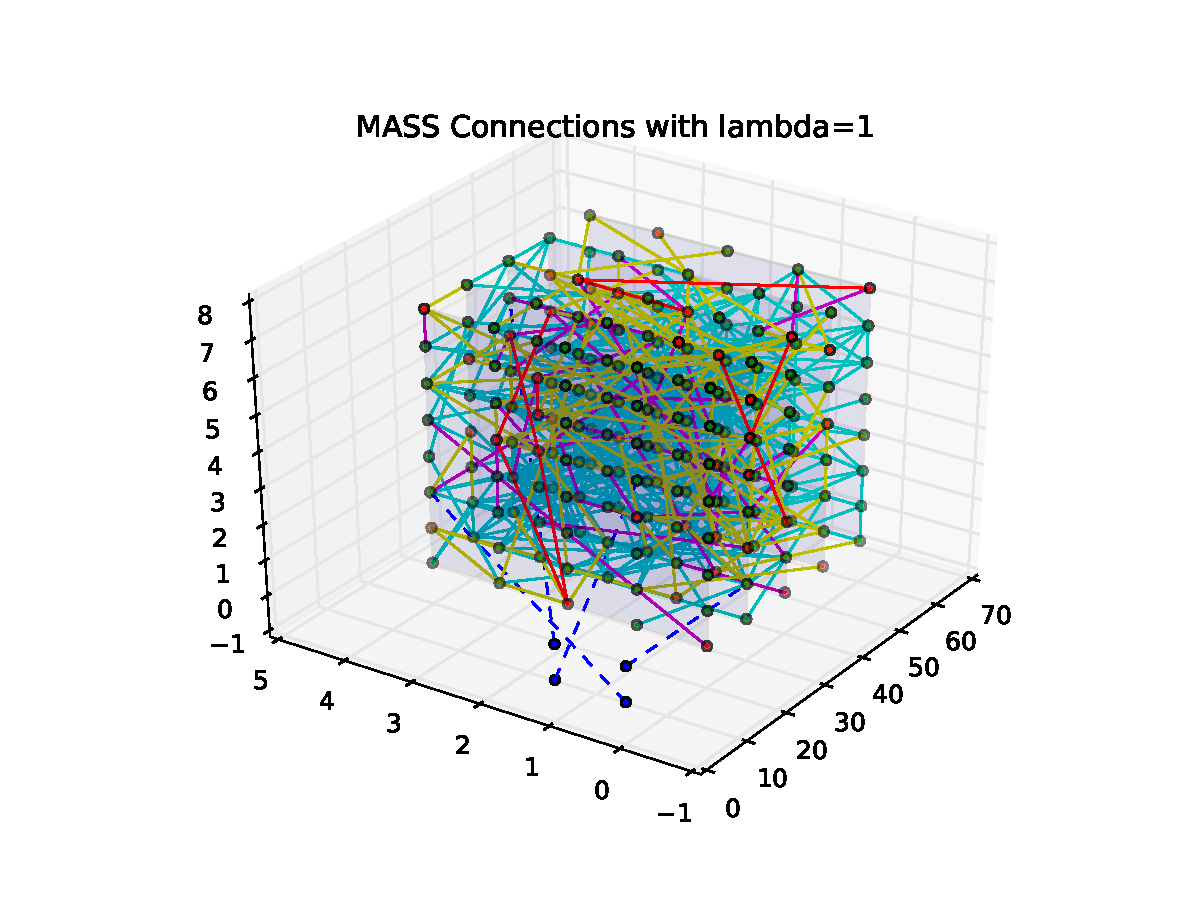
\includegraphics[height=6.0cm]{maas_lamb_1}
	 \label{fig:maas_lamb_1}
}
\subfloat[توپولوژی \lr{Maas} با $\lambda=1.5$]{
	 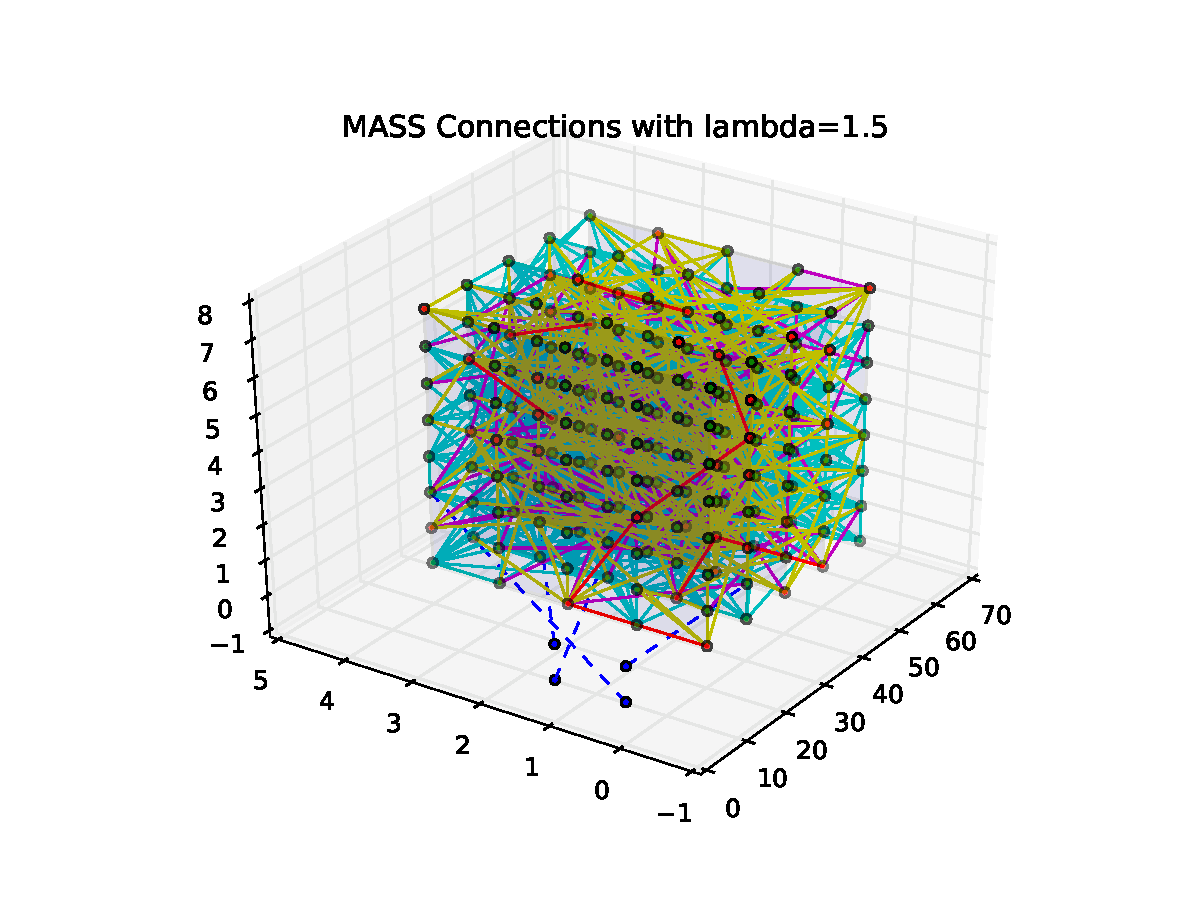
\includegraphics[height=6.0cm]{maas_lamb_15}
	  \label{fig:maas_lamb_15}
}

\caption[اتصالات در توپولوژی \lr{Maas}]{اتصالات در توپولوژی \lr{Maas}: با افزایش $\lambda$ تعداد و تراکم اتصالات افزایش می‌یابد}
\label{fig:maas}
}
\end{figure}

که در آن $\lambda$ پارامتر اتصال و $D(a,b)$ فاصله‌ی اقلیدسی بین دو نورون $a$ و $b$ است. $C$ بسته به نوع نورون پیش و پس‌سیناپسی مشخص می‌شود و ما اینجا مقادیر مشابه مقاله‌ی Maas \cite{maass2002real} را استفاده کرده‌ایم که بر مبنای اندازه‌گیری‌ها و مشاهدات سیناپسی روی قشر مغز یافت شده است\cite{gupta2000organizing}: $C$ برای اتصال تحریکی به تحریکی (EE) برابر $0.3$، تحریکی به مهاری (EI) برابر $0.2$، مهاری به تحریکی (IE) برابر $0.4$ و مهاری به مهاری (II) برابر $0.1$ قرار می‌گیرد. در این حالت اتصال، شکل فضایی اتصالات کروی و به صورت شعاعی صورت گرفته و از این رو جهت مطرح نیست. شکل \ref{fig:maas} افزایش تراکم اتصالات با افزایش $\lambda$ را به تصویر می‌کشد. طبق این مدل، اتصالات در یک شعاع مدور از نورون پیش‌سیناپسی قرار می‌گیرند و ارجحیت به یک جهت خاص وجود ندارد. در اینجا عملکرد این روش اتصال  بر مبنای مقادیر مختلف تراکم اتصالات $\lambda$ و  ضریب وزن $W_{scale}$ مورد بررسی قرار گرفته است.

\subsubsection{شبکه‌های دنیای کوچک}
یک شبکه‌ی دنیای کوچک\cite{watts1998collective} نوعی گراف است که دو خصوصیت دارد: (۱) گره‌ها (نورون‌ها) نسبت به یک گراف تصادفی بسیار خوشه‌بندی شده‌اند و (۲) بین هر دو گره در شبکه، مسیری با طول کوتاه وجود دارد. نشان داده شده است که بسیاری از شبکه‌های جهان واقعی نه کاملا نظم و ترتیب داشته و نه صرفا تصادفی هستند، بلکه خصوصیات دنیای کوچک را از خود نشان می‌دهند. یک شبکه‌ی دنیای کوچک را می‌توان با سیم‌کشی مجدد اتصالات یک شبکه با ساختار مشبک\footnote{\lr{Lattice}} به دست آورد. روش‌های سیم‌کشی مجدد مختلفی وجود دارند که خصوصیات دنیای کوچک را از خود نشان می‌دهند. 

\begin{figure}
\centering
{\footnotesize
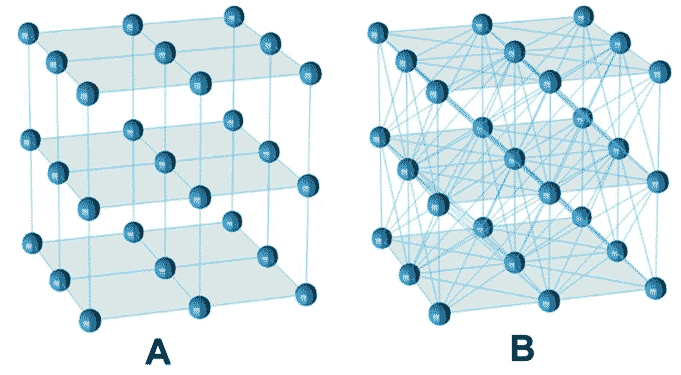
\includegraphics[height=5.5cm]{1_lattices}
\caption[مشبک‌های استفاده شده برای ساخت شبکه‌های دنیای کوچک]{مشبک‌های استفاده شده برای ساخت شبکه‌های دنیای کوچک. در مشبک (A) برای راس میانی ۶ اتصال خروجی و ۶ اتصال ورودی وجود دارد. ضریب خوشه‌گرایی آن صفر است زیرا اتصالی بین همسایه‌های گره‌ها وجود ندارد. مشبک (B) برای راس میانی ۲۶ اتصال ورودی و خروجی دارد.}
\label{fig:lattices}
}
\end{figure}

متوسط طول کوتاه‌ترین مسیر نمایانگر متوسط تعداد یال‌هایی است که باید برای رفتن از یک گره به گره‌ی دیگر پیموده شود (خاصیت سراسری\footnote{\lr{Global property}}). همچنین متوسط ضریب خوشه‌گرایی میزان همبندی موجود در شبکه را اندازه‌گیری می‌کند (خاصیت محلی\footnote{\lr{Local property}}).

طول کوتاهترین مسیر بین هر دو گره در فیلتر مایع با محاسبه‌ی حداقل تعداد سیناپس‌هایی که باید برای رفتن از یک نورون به نورونی دیگر طی شود بدست می‌آید. متوسط طول کوتاهترین مسیر با میانگین گرفتن طول کوتاهترین مسیر برای هر زوج نورون در کل شبکه‌ی فیلتر مایع محاسبه می‌گردد. ضریب خوشه‌گرایی برای هر نورون، تعداد اتصالات با همسایه‌هایش (به جز خودش)، تقسیم بر تعداد کل سیناپس‌های ممکن است. متوسط ضریب خوشه‌گرایی با میانگین گرفتن ضرایب خوشه‌گرایی برای همه‌ی نورون‌های شبکه به دست می‌آید. 

فیلتر مایع در اینجا شامل ۲۰۰ نورون \lr{LIF} است که در یک مشبک با ابعاد $5\times5\times8$ قرار گرفته‌اند. ما دو نوع ساختار اتصال مشبک را بررسی کرده‌ایم (شکل \ref{fig:lattices}). اتصالات بین نورون‌ها در ابتدا بر اساس یکی از دو مشبک ساخته می‌شوند. پس از ساخت فیلتر مایع مشبک، هر سیناپس با احتمال $P$ به صورت تصادفی به نورونی دیگر سیم‌کشی جایگزین می‌شود؛ با این قید که حلقه و اتصالات موازی (چند اتصال با نورون پیش و پس‌سیناپسی یکسان) مجاز نمی‌باشد. دقت کنید که عملیات سیم‌کشی مجدد مجموع تعداد سیناپس‌ها در فیلتر مایع را تغیر نمی‌دهد. مشبک (A) تعداد $989$ سیناپس ($639$ اتصال \lr{EE}، $155$ اتصال \lr{EI}، $155$ اتصال \lr{IE} و $40$ اتصال \lr{II}) و مشبک (B) تعداد $3494$ سیناپس ($2271$ اتصال \lr{EE}، $541$ اتصال \lr{EI}، $546$ اتصال \lr{IE} و $137$ اتصال \lr{II}) برقرار می‌کند (شکل \ref{fig:sw}). با افزایش احتمال سیم‌کشی مجدد $P$، ارتباطات سیناپسی با برد طولانی‌تر ایجاد شده و متوسط طول کوتاهترین مسیر به شدت کاهش می‌یابد. اگر $P$ برابر یک قرار گیرد، فیلتر مایع به یک شبکه‌ی کاملا تصادفی تغییر ماهیت می‌دهد. در ادامه عملکرد این مدل را بر حسب مقادیر مختلف احتمال $P$ و ضریب وزنی $W_{scale}$برای دو مشبک اتصال مذکور مورد بررسی قرار خواهیم داد.


\begin{figure}
\centering
{\footnotesize
\subfloat[توپولوژی \lr{SW}  نوع \lr{A} با $P=0$]{
	 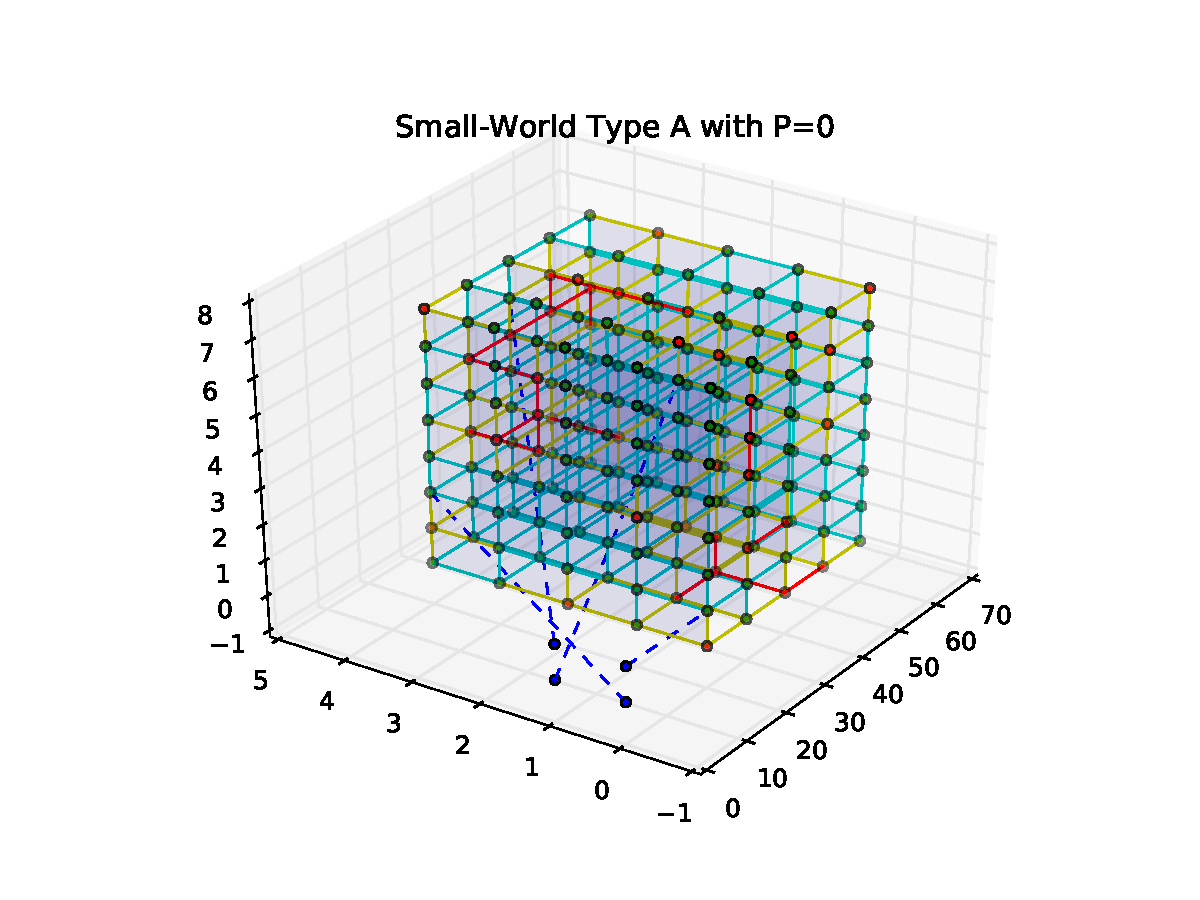
\includegraphics[height=6.0cm]{sw_a_0}
	 \label{fig:sw_a_0}
}
\subfloat[توپولوژی \lr{SW}  نوع \lr{B} با $P=0$]{
	 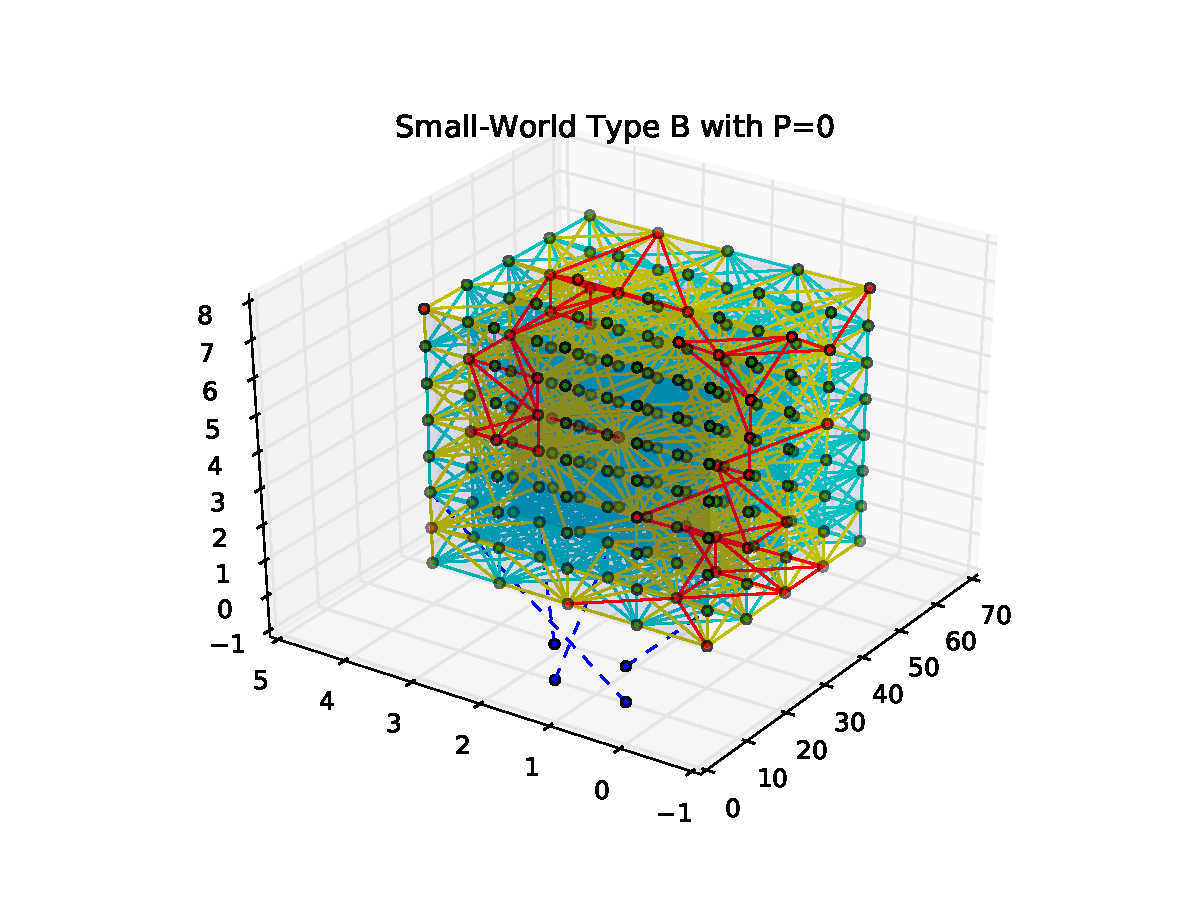
\includegraphics[height=6.0cm]{sw_b_0}
	  \label{fig:sw_b_0}
}

\subfloat[توپولوژی \lr{SW}  نوع \lr{A} با $P=0.1$]{
	 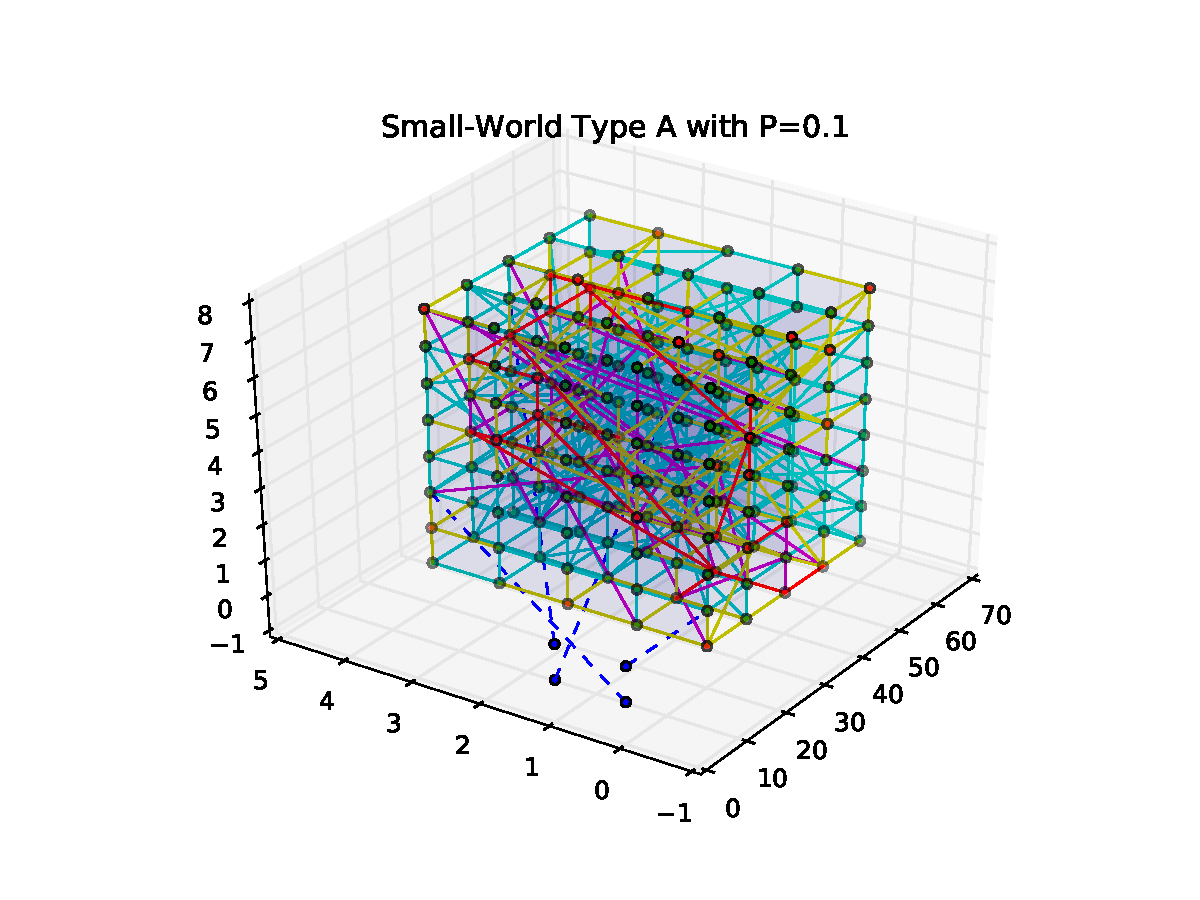
\includegraphics[height=6.0cm]{sw_a_01}
	 \label{fig:sw_a_0}
}
\subfloat[توپولوژی \lr{SW}  نوع \lr{B} با $P=0.1$]{
	 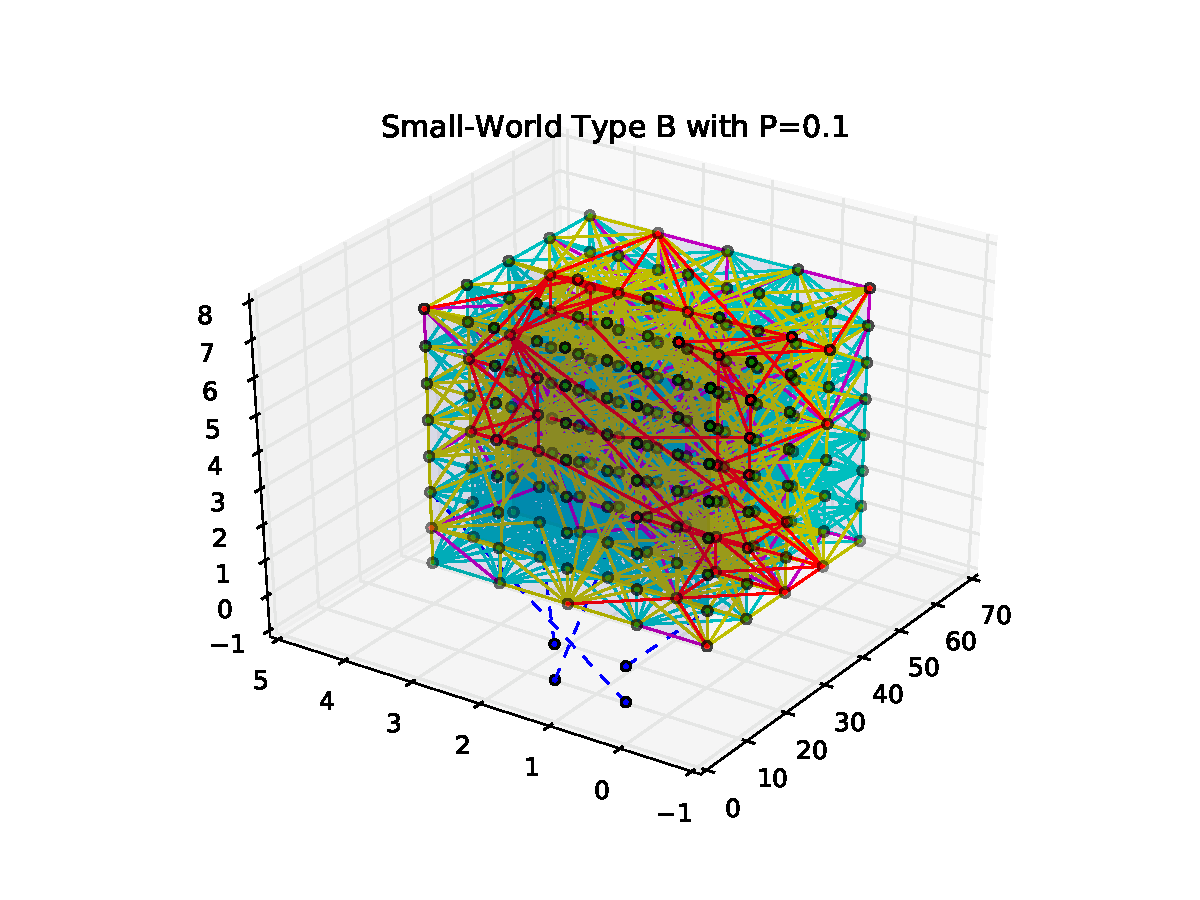
\includegraphics[height=6.0cm]{sw_b_01}
	  \label{fig:sw_b_0}
}
\caption[اتصالات در توپولوژی دنیای کوچک]{اتصالات در توپولوژی دنیای کوچک: با افزایش $P$ تعداد کل اتصالات ثابت باقی می‌ماند اما مشبک از حالت منظم خارج شده و اتصالات کوتاه تصادفی بین نورون‌ها حایگزین می‌شود.}
\label{fig:sw}
}
\end{figure}

%
%\subsubsection{مدل آکسون}
%مخروط رشد آکسون یک خط مستقیم را دنبال می‌کند مگر اینکه راهنما وجود داشته یا اینکه گذرگاه بسته باشد\cite{yamamoto2002wiring}. شبیه‌سازی‌های پیشین \cite{kaiser2009simple} نشان می‌دهد که با استفاده از یک قاعده‌ی ساده‌ی رشد مستقیم آکسون‌ها در جهت‌های تصادفی در فضای ۲بعدی و تراکم نورونی حدود ۴٪ می‌توان به توزیع طول اتصال مشابهی با آنچه به صورت تجربی در مغز موش و کرم الگانس\footnote{\lr{Caenorhabditis elegans}} مشاهده شده است رسید. در راستای همین تحقیق، در اینجا نیز با قرار دادن تعداد ؟؟؟ نورون در موقعیت‌های صحیح از یک فضای سه بعدی به ابعاد ??x??x?? این کار صورت گرفته است که تراکم نورونی ؟؟٪ را می‌دهد. برای هر نورون یک بردار تصادفی به عنوان جهت رشد آکسونی آن تولید می‌شود. طبق فرض صورت گرفته، آکسون‌ها در یک مسیر مستقیم رشد می‌کنند تا زمانی که به لبه‌ی بردار مایع برخورد کنند. از آنجایی که هر نورون یک فضای دارینه‌ی متناهی دارد که تعداد ارتباطات سیناپسی را محدود می‌کند، جاهای خالی برای اتصالات پیش و پس‌سیناپسی محدود می‌شوند: اگر جاهای خالی هم پیش و هم پس‌سیناپسی پر شوند، اتصال ورودی یا خروجی دیگری امکان برقرار شدن ندارد. اتصال از نورون A به نورون B تنها در حالی تشکیل می‌شود که فاصله‌ی آکسون بین‌آنها از $R$ واحد کمتر بوده و همچنین نورون A حداقل یک جای خالی پس‌سیناپسی و نورون B حداقل یک جای خالی پیش‌سیناپسی داشته باشند. آکسون‌ها به ترتیب تصادفی یکی پس از دیگری ساخته می‌شوند. از این رو، نورون‌هایی که آکسون‌هایش زودتر ساخته می‌شوند این مزیت را دارند که به هر نورونی که می‌خواهند متصل گردند در حالی که نورون‌هایی که اتصالاتشان دیرتر تشکیل می‌شود باید به اجبار به صورت انتخابی عمل کرده و ارتباطاتشان را محدود به نورون‌هایی کنند که هنوز جای خالی دارند.
%
%یک حد پایین جاهای خالی پیش و پس‌سیناپسی باعث رقابت بین نورون‌ها برای جاهای خالی پیش‌ و پس‌سیناپسی می‌شود. حد جاهای خالی پیش و پس‌سیناپسی به ترتیب روی ۱۵ و ۳۰ قرار داده شده‌اند. در این ساختار، اتصالات خروجی بر خلاف روش اصلی که به صورت شعاعی عمل می‌کرد، به صورت جهت‌دار ساخته می‌شوند. برد اتصالات خروجی هر نورون شکل سیلندری با شعاع $R$ دارد. 
%
%از آنجایی که طول اتصالات بین نورون‌ها مشابه توصیه منطبق بر زیست‌شناسی است\cite{kaiser2009simple}، مطلوب است که طول اتصالات در نتیجه‌ی شبیه‌سازی تاثیر بگذارد. سرعت انتشار ضربه در طول آکسون ثابت است، از این رو آکسون‌های طولانی‌تر تاخیر‌های طولانی‌تری را باعث می‌شوند. به این جهت ما نیز تاخیر هر سیناپس را به نسبت فاصله‌ی اقلیدسی بین دو نورون پیش و پس‌سیناپسی تعیین می‌کنیم تا آکسون‌های طولانی، تاخیر بیشتری داشته باشند. 

\section{نتایج}
\subsection{میزان تفکیک‌پذیری}
پیش از آنکه به بررسی طبقه‌بندهای مختلف برای لایه‌ی قرائت پرداخته شود، به ارائه‌ی معیاری تحت عنوان میزان تفکیک‌پذیری\footnote{\lr{Separation measure}} می‌پردازیم. اشکال استفاده از عملکرد لایه‌ی قرائت برای ارزیابی شبکه این است که می‌تواند از لحاظ محاسباتی زمان‌بر باشد. علاوه بر آن استفاده از عملکرد لایه‌ی قرائت روشی غیر مستقیم برای اندازه‌گیری عملکرد فیلتر مایع است زیرا به واقع عملکرد لایه‌ی قرائت، و نه فیلتر مایع، را مورد سنجش قرار می‌دهد و از این روی قدرت و ضعف ساز و کار استفاده شده در لایه‌ی قرائت می‌تواند به برداشت نادرستی از توان فیلتر مایع بیانجامد. به همین جهت از خاصیت تفکیک‌پذیری استفاده می‌شود که می‌تواند دید خوبی از توانایی جداسازی الگوهای مختلف توسط شبکه به ما دهد. استفاده از یک معیار مناسب که بتواند با استفاده از میانگین‌ها و پراش‌های داده‌ها قدرت تفکیک‌پذیری شبکه را ترسیم کند بسیار مهم است. عموم کارهای منتشر شده در ارتباط با ماشین حالت مایع از نرخ افتراقی فیشر\footnote{\lr{Fisher Discriminant Ratio}}(\lr{FDR})\cite{fisher1936use} به عنوان معیار میزان تفکیک‌پذیری استفاده می‌کنند\cite{hourdakis2011improving,ju2013effects} که شرح آن در ادامه می‌آید. برای روش \lr{FDR}، دو ماتریس پراکندگی بین کلاسی و پراکندگی میان‌کلاسی را به ترتیب طبق فرمول‌های \ref{eq:s_b} و \ref{eq:s_w} محاسبه می‌کنیم.

\begin{equation}\label{eq:s_b}
S_b = \sum_{i=1}^{M}P_i(\mu_i-\mu_0)(\mu_i-\mu_0)^T
\end{equation} 
\begin{equation}\label{eq:s_w}
S_w = \sum_{i=1}^{M}P_i\Sigma _i
\end{equation} 
که در آنها $\mu_0 = \sum_{i=1}^{M}P_i\mu_i$ میانگین سراسری برای همه $M$ کلاس (۲ کلاس در اینجا)، $P_i$ احتمال پیشین کلاس $\omega_i$ (در اینجا $0.5$) و $\mu_i$ میانگین حالت‌های مایع\footnote{\lr{Liquid States}} متناظر با کلاس $\omega_i$ است.همچنین $\Sigma _i$  ماتریس همبستگی حالت‌های مایع کلاس $\omega_i$ است.

سپس ماتریس همبستگی $S_m$ به صورت زیر تشکیل می‌گردد:
\begin{equation} 
S_m = S_w + S_b
\end{equation} 
اثر\footnote{\lr{Trace}} ماتریس $S_m$ می‌تواند مجموع پراش\footnote{\lr{Variance}} ویژگی‌ها را حول میانگین سراسری حساب کند در حالی که اثر $S_w$ مجموع پراش ویژگی‌ها برای همه‌ی کلاس‌ها می‌باشد. در نتیجه میزان تفکیک‌پذیری بین کلاس‌ها را می‌توان بر حسب کمیت تعریف شده در \ref{eq:fdr} بیان کرد:
\begin{equation}\label{eq:fdr}
FDR = trace\left \{ S^{-1}_w S_m \right \}
\end{equation} 
با این حال در این تحقیق از این معیار استفاده نشده است. بدلیل هم‌خطی\footnote{\lr{Collinear}} بودن عملکرد برخی از نورون‌ها تحت حالات خاص از شرایطی که اینجا بررسی می‌شود، ماتریس $S_w$ ممکن است تکین\footnote{\lr{Singular}} شده و در نتیجه ماتریس وارون‌پذیر\footnote{\lr{Invertible}} نباشد. برای فائق آمدن بر این حالت می‌توان یک مقدار کوچک و قابل چشم‌پوشی به قطر ماتریس اضافه کرده و یا اینکه از شبه وارون\footnote{\lr{Pseudoinverse}} استفاده نمود. با این حال، با وجود اینکه از این روش‌ها می‌توان برای کاربردهایی مانند استفاده به عنوان برازش ماشین حالت مایع استفاده کرد، اما در اینجا بخاطر اهمیت مرتبه‌ی میزان تفکیک‌پذیری در ترسیم عملکرد شبکه بر حسب پارامتر‌های مختلف، از نرخ افتراقی فیشر استفاده نشده است.

معیارهای میزان تفکیک دیگری که بعضا در ادبیات موضوع استفاده شده است اغلب بر حسب توابع فاصله در ریاضیات مانند فاصله‌ی اقلیدسی\footnote{\lr{Euclidean distance}}\cite{grzyb2009model,norton2006preparing} یا فاصله‌ی بری-کرتیس\footnote{\lr{Bray-Curtis dissimilarity}}\cite{wojcik2015bray}
می‌باشند. بر اساس مدل‌های پیشین و یافته‌های مربوط، ما معیار زیر را جهت نمایش میزان تفکیک‌پذیری ارائه کرده‌ایم:

\begin{equation}\label{eq:betw}
D_b = \frac{\sum_{i=1}^{M}\sum_{j=1}^{M}\left \| \mu_i -\mu_j \right \|_2}{M^2},
\end{equation} 
که $D_b$ بر حسب تفاضل میانگین وضعیت نورون هر کلاس، $\mu_i$، امکان تمایز بین آنها را می‌سنجد و مشابه آن در برخی از کارها \cite{norton2006preparing} به عنوان معیار میزان تفکیک‌پذیری استفاده شده است. با حال این معیار در بررسی‌های صورت گرفته عملکرد خوبی نداشت و ما را به اضافه کردن فاکتور دیگری که نمایانگر نزدیکی حالات نمونه‌های متناظر با یک کلاس بود سوق داد:

\begin{equation}\label{eq:withi}
D_w = \sum_{i=1}^{M}\sum_{j=1}^{N}\delta_{i,j},
\end{equation} 
که در آن $D_w$ با محاسبه‌ی مجموع پراش نمونه‌های هر کلاس در میان خود، قرابت حالات ماشین حالت مایع را در مواجهه با نمونه‌های یکسان و عدم حساسیت آن به تغییرات جزئی و کوچک را نشان می‌دهد. در نهایت میزان تفکیک‌پذیری به صورت زیر تعریف می‌شود:
\begin{equation}\label{eq:separ}
Separation = \frac{D_b}{D_w+1}
\end{equation} 
که عدد یک در مخرج برای حالات معدودی هست که ممکن است واریانس بین نمونه‌ها وجود نداشته یا صرفا یک نمونه از یک کلاس وجود داشته باشد. طبق معیار ارائه شده اگر فاصله‌ی بین‌کلاسی بیش از فاصله‌ی میان‌کلاسی باشد، انتظار می‌رود یک طبقه‌بند خطی به نحو بهتری بتواند بین نمونه‌های ورودی تمایز قائل شود.

\begin{figure}
\centering
{\footnotesize
\subfloat[مدل \lr{Maas}]{
	 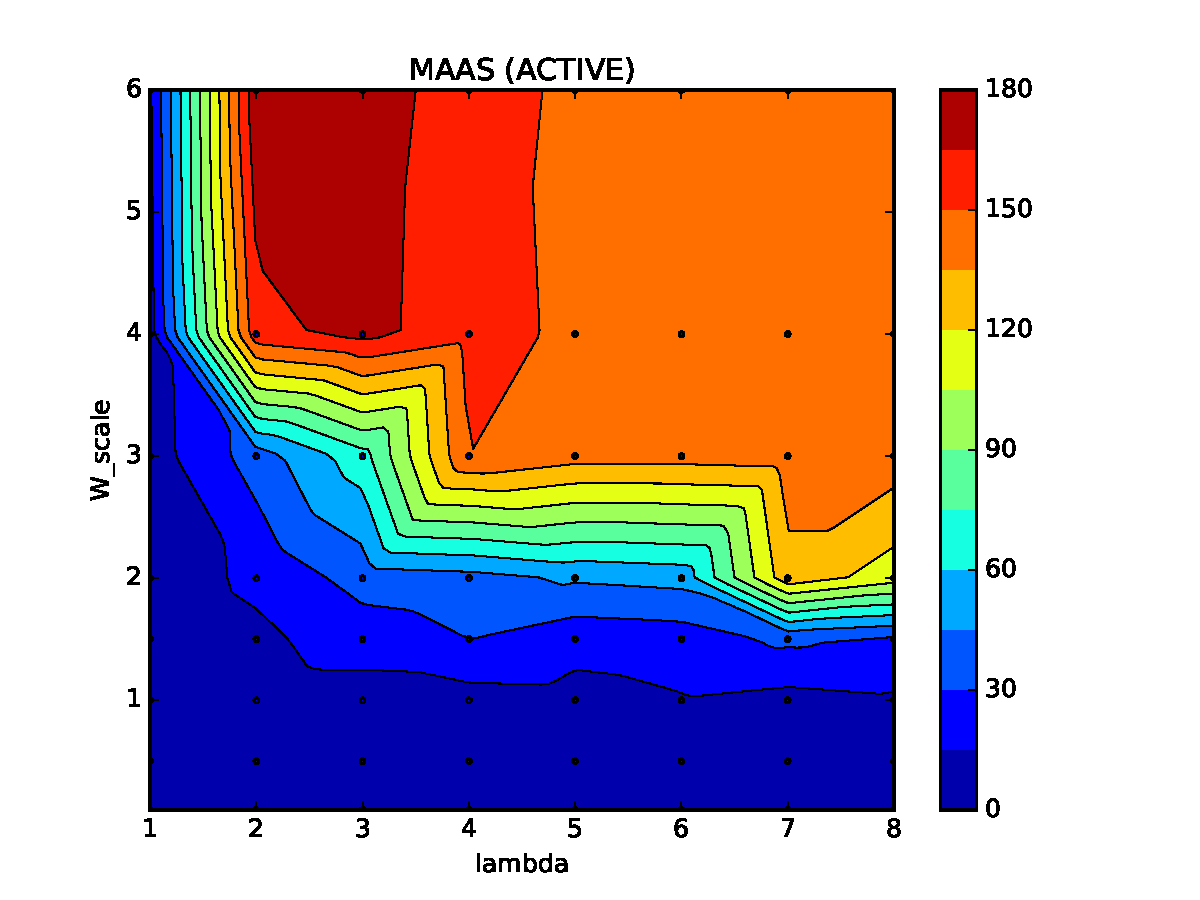
\includegraphics[height=6.0cm]{MAAS_LIQOUT--1_17_30-0_4_5--1_ACTIVE}
	 \label{fig:active_maas}
}

\subfloat[مدل \lr{SW-A}]{
	 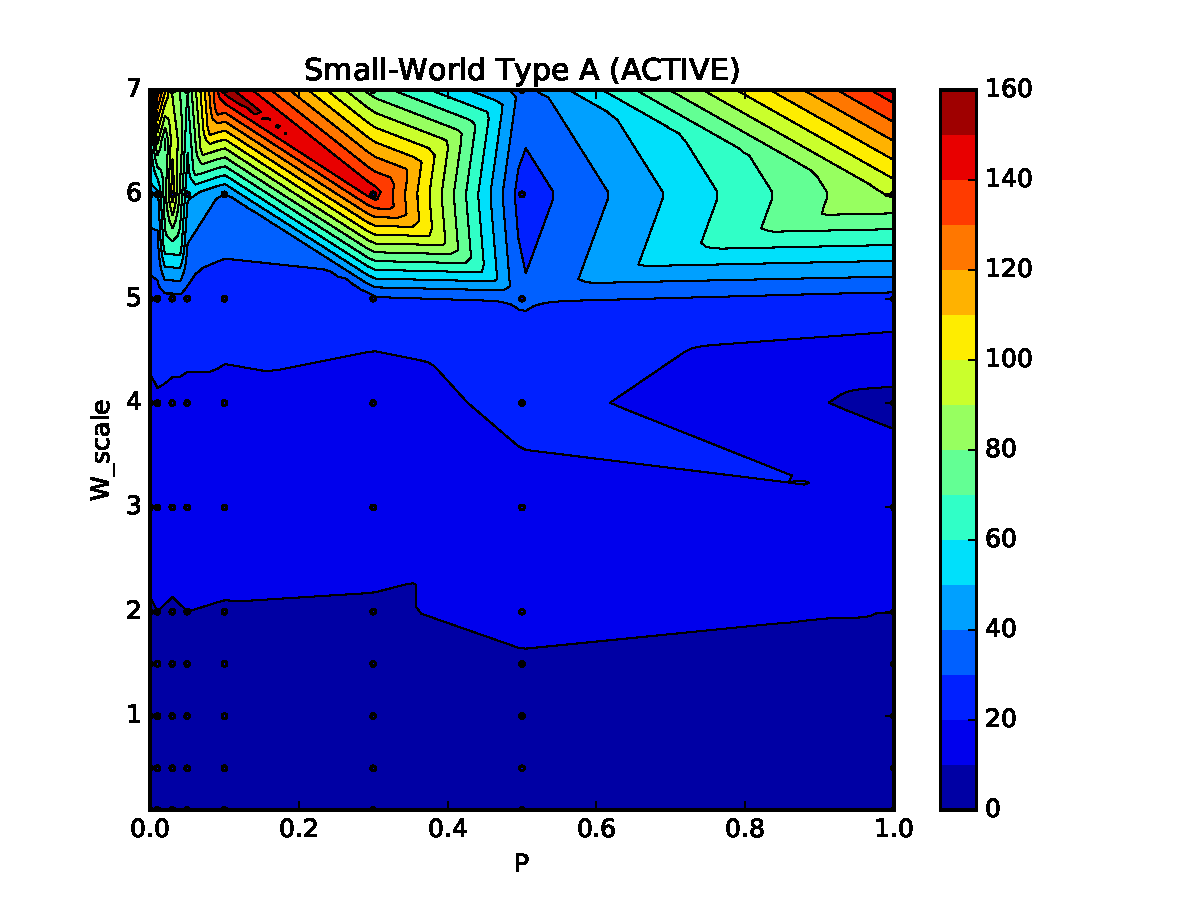
\includegraphics[height=6.0cm]{SW_LIQOUT--1_17_30-0_4_5--A_1_ACTIVE}
	  \label{fig:active_swa}
}
\subfloat[مدل \lr{SW-B}]{
	 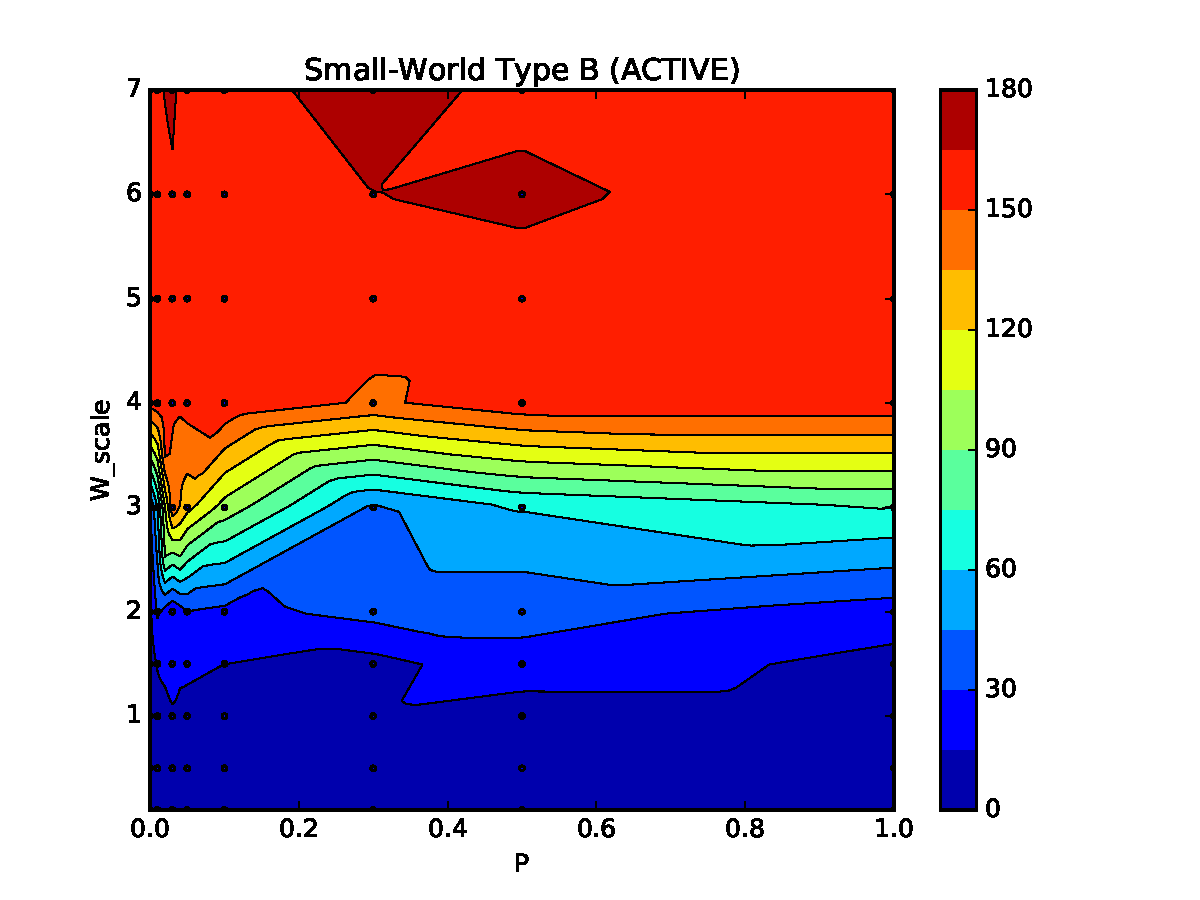
\includegraphics[height=6.0cm]{SW_LIQOUT--1_17_30-0_4_5--B_1_ACTIVE}
	 \label{fig:active_swb}
}
\caption[تعداد نورون‌های فعال برای مدل‌های اتصال]{تعداد نورون‌های فعال برای مدل اتصال \subref{fig:active_maas} \lr{Maas}، \subref{fig:active_swa} دنیای کوچک نوع \lr{A} و  \subref{fig:active_swb} دنیای کوچک نوع \lr{B}}
\label{fig:active}
}
\end{figure}

\section{نتایج}
جهت اینکه صرفا به ارزیابی توان محاسباتی فیلتر مایع پرداخته باشیم، نورون‌هایی که مستقیما ورودی را از شبکه‌ی سلسله مراتبی دریافت می‌کنند از ماتریس حالت فیلتر مایع حذف شده‌اند و در نتیجه بردار حالت \lr{LSM} از ۱۹۶ عنصر (به جای ۲۰۰ عنصر) تشکیل شده است. در این بخش به بررسی عملکرد ماشین حالت مایع برای سه نوع اتصال سیناپسی (مدل \lr{Maas} و مدل دنیای کوچک \lr{A} و \lr{B}) تحت معیار میزان تفکیک‌پذیری و همچنین طبقه‌بندهای خطی می‌پردازیم. برای نتایج گزارش شده، شبکه به ازای هر مجموعه پارامتر، شش بار اجرا شده و میانگین نتایج برآمده از این اجراها به عنوان نتیجه گزارش شده است. در بخش‌های زیادی از شبیه‌سازی (همانند وزن‌های اولیه و اتصالات سیناپسی) از اعداد تصادفی بدست آمده توسط یک تابع مولد اعداد شبه‌تصادفی\footnote{\lr{Pseudorandom number generator}} استفاده شده است که با تنظیم بذر\footnote{\lr{Seed}} روی شش مقدار مختلف، امکان تولید شبکه‌های مختلف به ازای یک پارامتر که امکان بازتولید نیز داشته باشند فراهم شده است.

ضریب وزن سیناپسی $W_{scale}$ مدل \lr{Maas} به ازای مقادیر  $0.5$، $1$، $1.5$، $2$، $3$، $4$ و $6$ و پارامتر تراکم اتصالات $\lambda$ به ازای مقادیر $1$، $2$، $3$، $4$، $5$، $6$، $7$ و $8$ مورد بررسی قرار گرفته است. برای مدل اتصال دنیای کوچک، ضریب وزن به ازای مقادیر $0.1$، $0.5$، $1$، $1.5$، $2$، $3$، $4$، $5$، $6$ و $7$ و همچنین پارامتر احتمال سیم‌کشی مجدد $P$ به ازای مقادیر  $0$، $0.01$، $0.03$، $0.05$، $0.1$، $0.3$، $.5$ و $1$ مورد بررسی قرار گرفته است. شکل‌های \ref{fig:active}، \ref{fig:separation}، \ref{fig:lda} و \ref{fig:svm} با درون‌یابی\footnote{\lr{Interpolation}} نقاط موجود ترسیم شده‌اند.

\subsection{میزان تفکیک‌پذیری}
شکل \ref{fig:separation} عملکرد ماشین‌های حالت مایع را براساس معیاری که پیشتر تحت عنوان میزان تفکیک‌پذیری ارائه شد نمایش می‌دهد. پارامتر $W_{scale}$ میزان انتقال سیگنال درون شبکه را می‌تواند تعیین کند. از جهت زمانی اگر مقدار بزرگی برای آن تعیین گردد، نورون‌های بیشتری آتش می‌کنند و اگر مقدار کوچکی برای آن تعیین گردد ممکن است هیچ کدام از نورون‌ها (به جز نورون‌های متصل به خروجی شبکه‌ی سلسله مراتبی) آتش نکنند. 


\begin{figure}
\centering
{\footnotesize
\subfloat[مدل \lr{Maas}]{
	 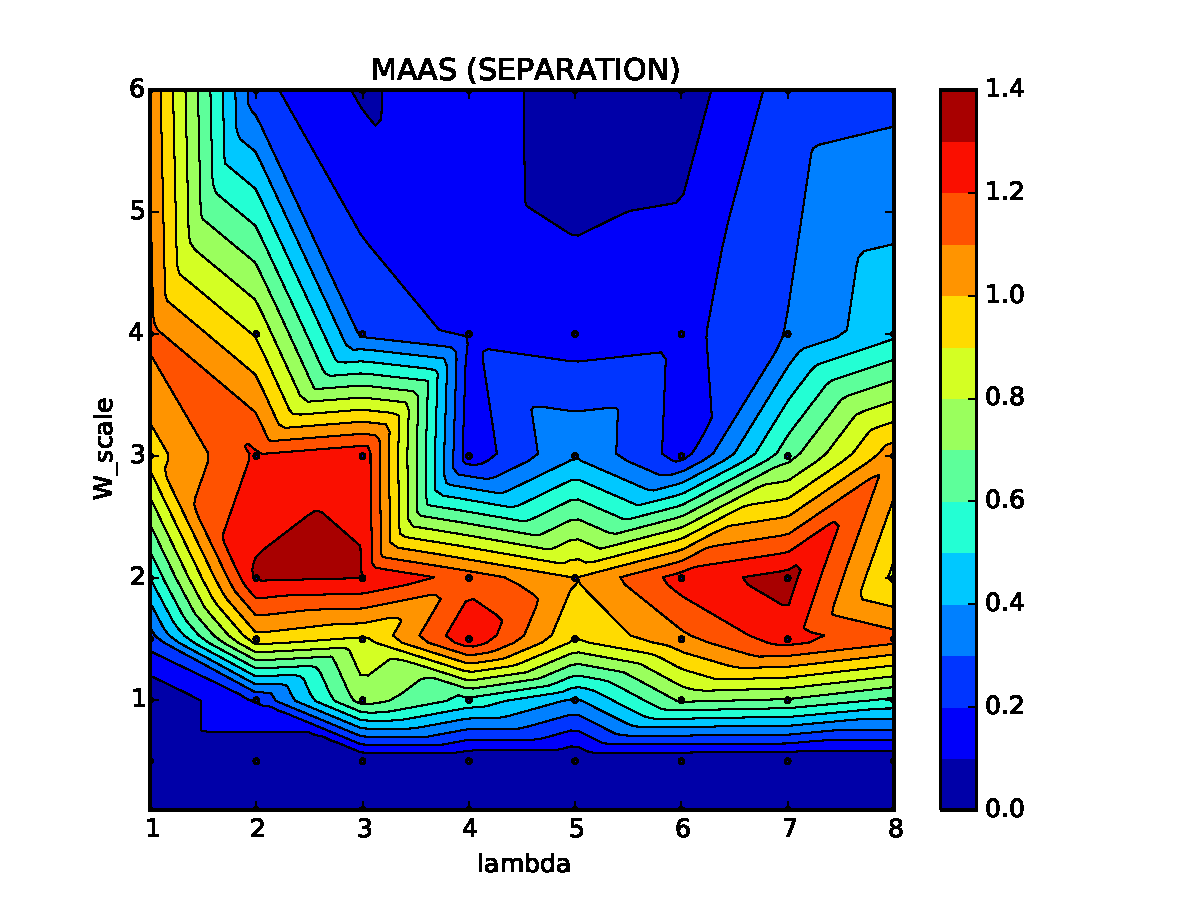
\includegraphics[height=6.0cm]{MAAS_LIQOUT--1_17_30-0_4_5--1_SEPARATION}
	 \label{fig:separation_maas}
}

\subfloat[مدل \lr{SW-A}]{
	 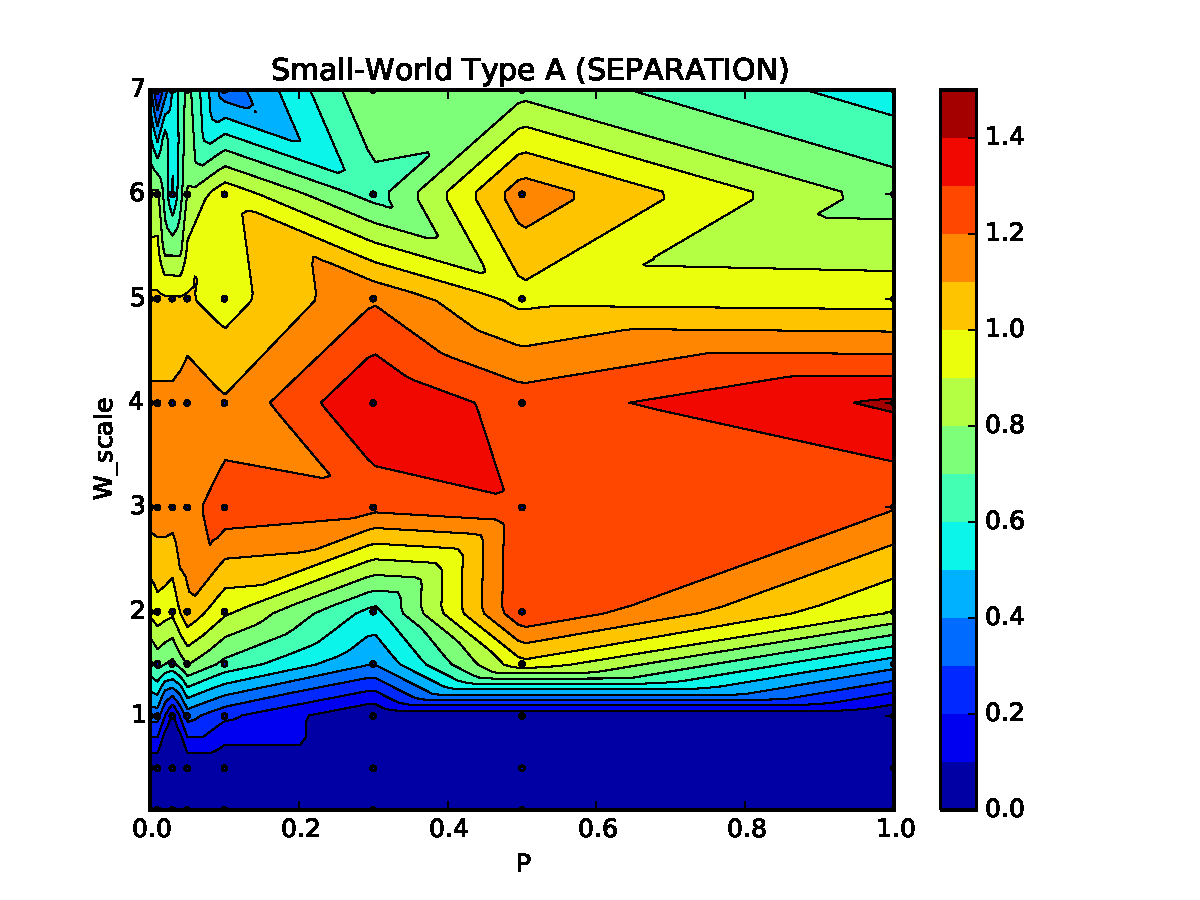
\includegraphics[height=6.0cm]{SW_LIQOUT--1_17_30-0_4_5--A_1_SEPARATION}
	  \label{fig:separation_swa}
}
\subfloat[مدل \lr{SW-B}]{
	 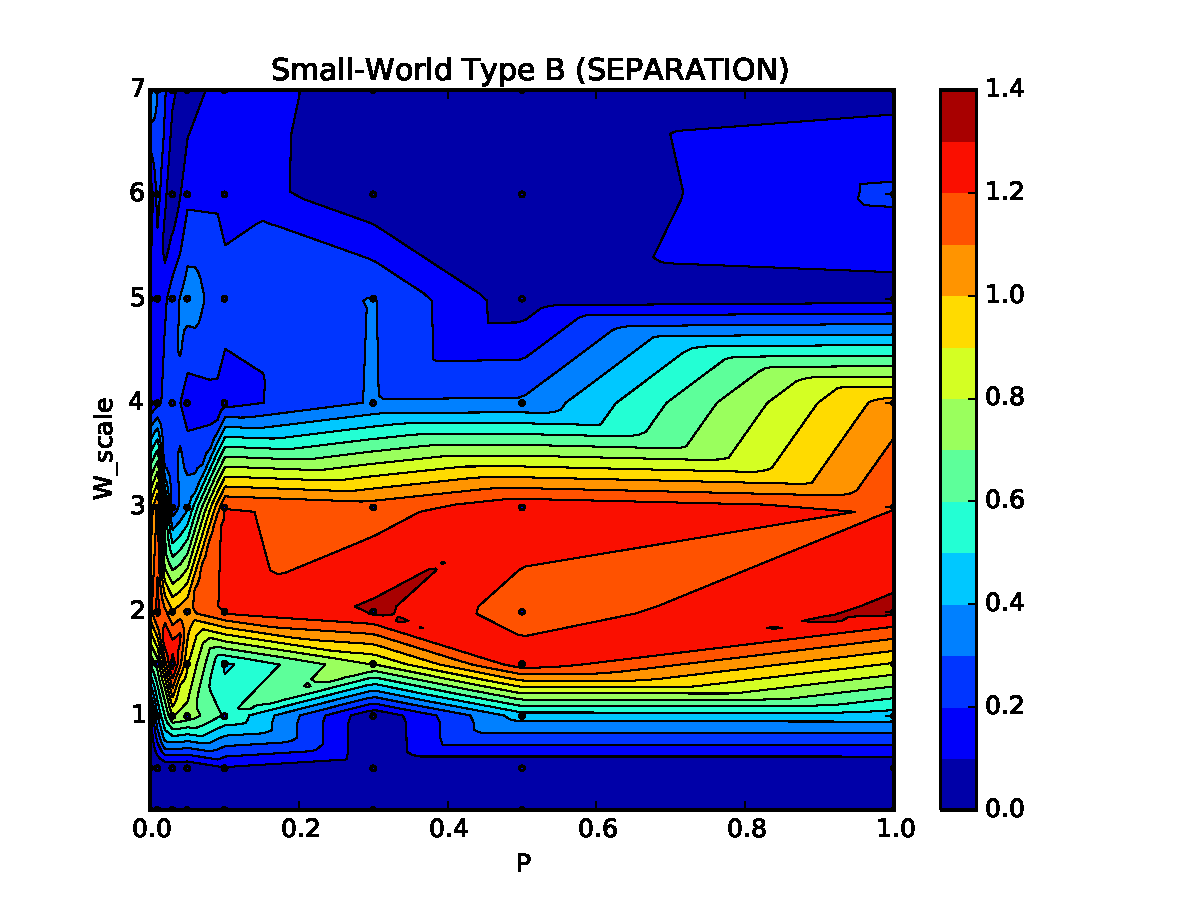
\includegraphics[height=6.0cm]{SW_LIQOUT--1_17_30-0_4_5--B_1_SEPARATION}
	 \label{fig:separation_swb}
}
\caption[میزان تفکیک‌پذیری برای مدل‌های اتصال]{معیار میزان تفکیک‌پذیری برای مدل اتصال \subref{fig:separation_maas} \lr{Maas}، \subref{fig:separation_swa} دنیای کوچک نوع \lr{A} و  \subref{fig:separation_swb} دنیای کوچک نوع \lr{B}}
\label{fig:separation}
}
\end{figure}

اتصالات سیناپسی، کانال‌های ارتباطی بین نورون‌ها هستند. با افزایش تعداد کانال‌های ارتباطی، نورون‌ها مسیرهای بیشتری برای ارتباط با یکدیگر دارند و در نتیجه میانگین طول کوتاهترین مسیر کاهش می‌یابد. 


\subsection{آنالیز افتراقی خطی}
شکل \ref{fig:lda} عملکرد ماشین‌های حالت مایع را براساس توانایی تمایز نمونه‌های دو کلاس توسط طبقه‌بند \lr{LDA} نمایش می‌دهد. آنالیز افتراقی خطی حاصل تعمیم روش افتراق خطی فیشر است که به موجب آن ترکیبی خطی از ویژگی‌ها حاصل می‌شود که قرار است به بهترین نحو نمونه‌های دو کلاس را از یکدیگر جدا کند. همانطور که در تصویر \ref{fig:lda} مشاهده می‌شود، برای برخی پارامتر‌های خاص مقداری گزارش نشده است. این امر از آن جهت است که بخاطر هم‌خطی بودن ستون‌های ویژگی که در شرایط خاصی مانند فقدان فعالیت نورونی (هنگامی که وزن‌های سیناپسی کوچک باشد) بوجود می‌آید، امکان اعمال آنالیز افتراقی خطی وجود ندارد.

\begin{figure}
\centering
{\footnotesize
\subfloat[مدل \lr{Maas}]{
	 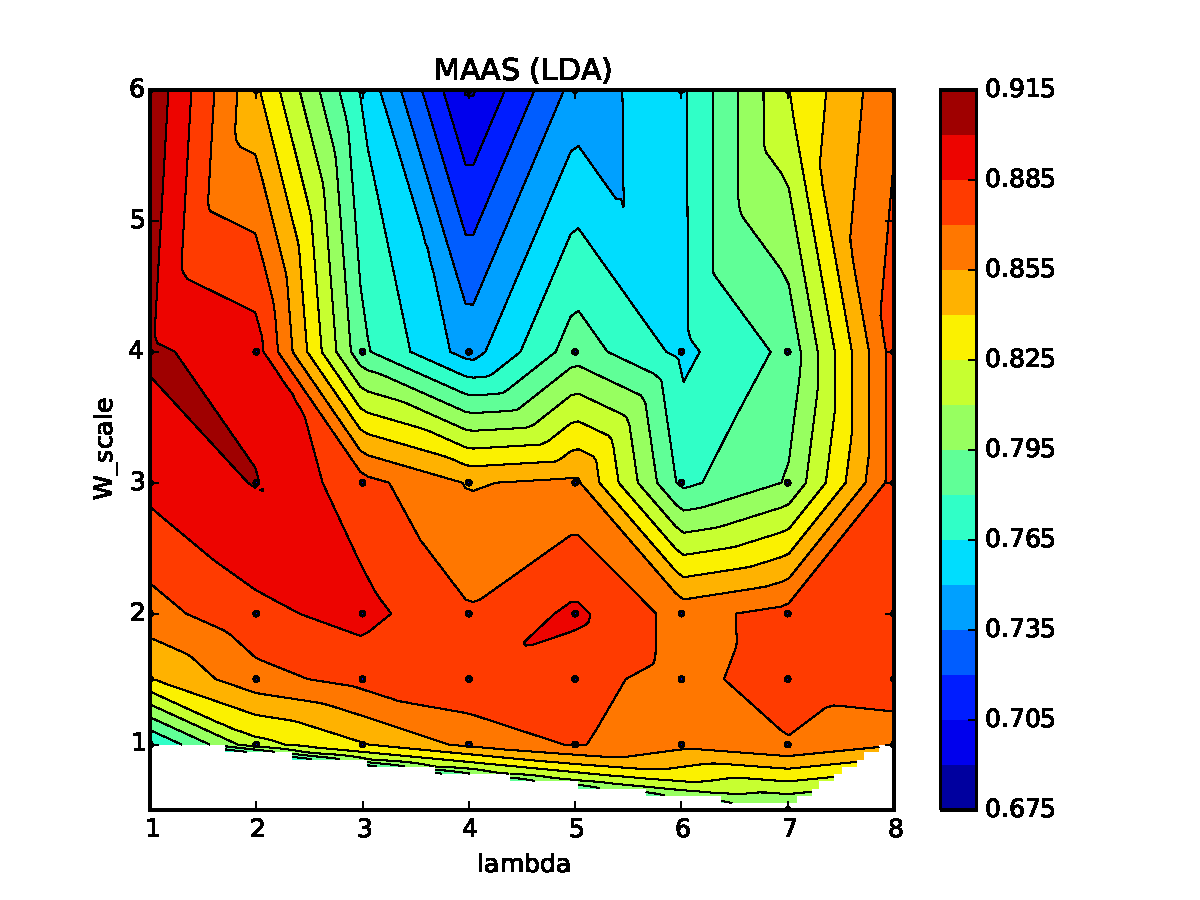
\includegraphics[height=6.0cm]{MAAS_LIQOUT--1_17_30-0_4_5--1_LDA}
	 \label{fig:lda_maas}
}

\subfloat[مدل \lr{SW-A}]{
	 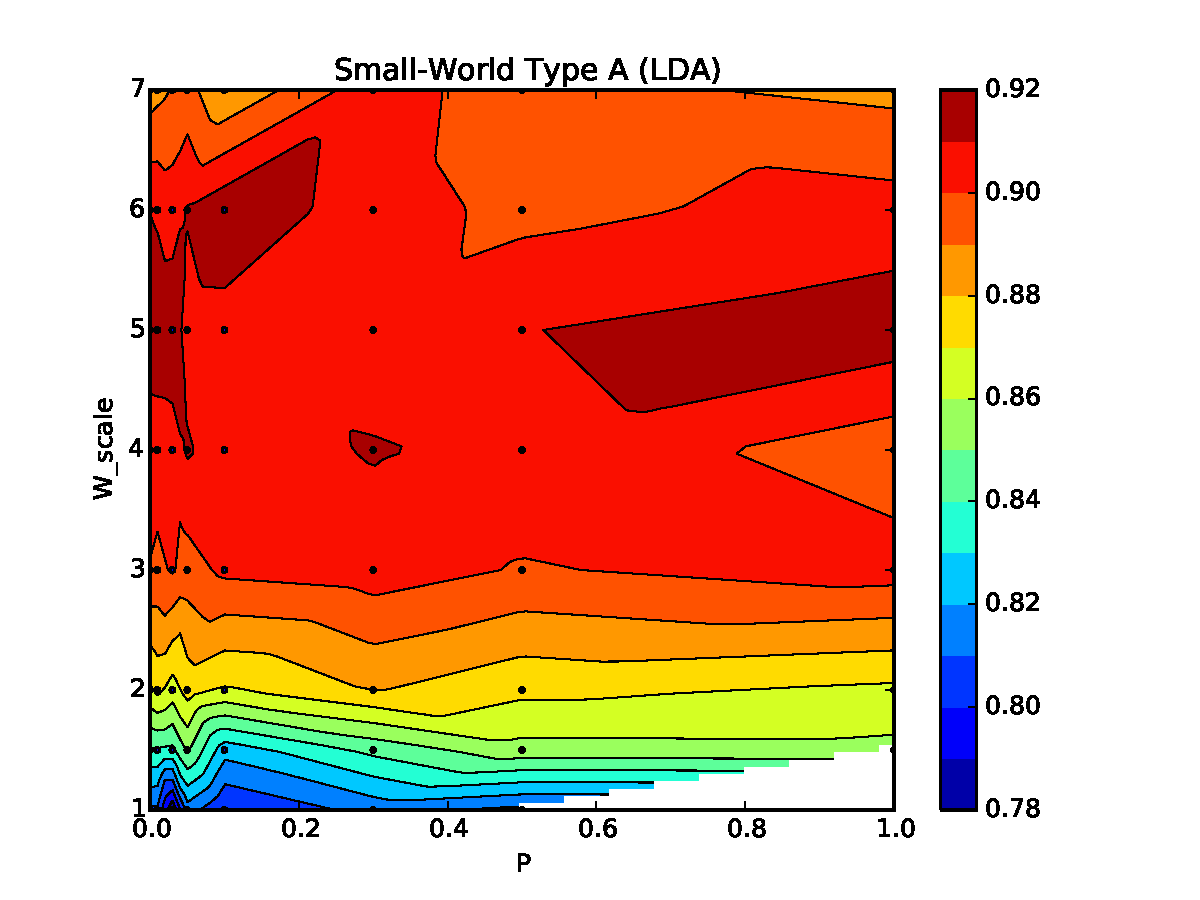
\includegraphics[height=6.0cm]{SW_LIQOUT--1_17_30-0_4_5--A_1_LDA}
	  \label{fig:lda_swa}
}
\subfloat[مدل \lr{SW-B}]{
	 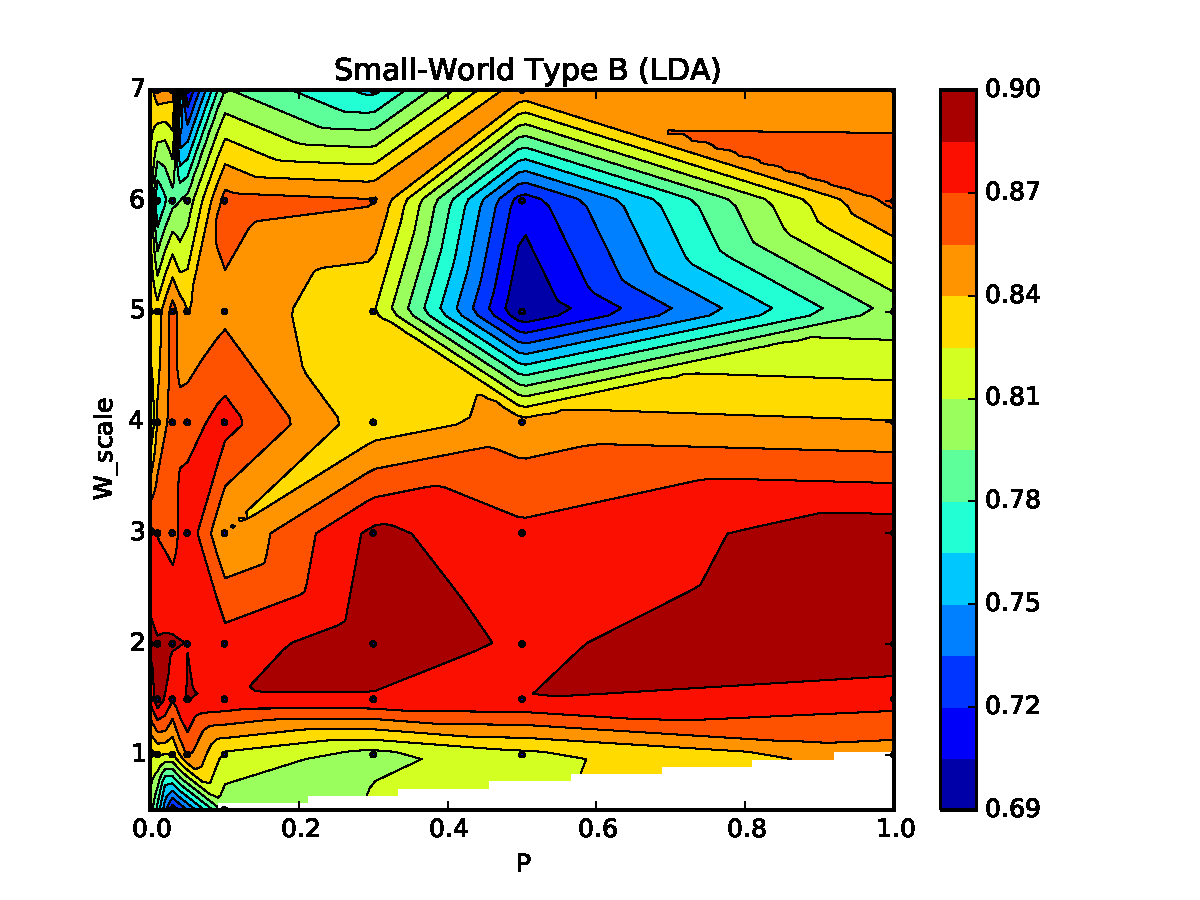
\includegraphics[height=6.0cm]{SW_LIQOUT--1_17_30-0_4_5--B_1_LDA}
	 \label{fig:lda_swb}
}
\caption[عملکرد طبقه‌بند \lr{LDA} برای مدل‌های اتصال]{عملکرد طبقه‌بند \lr{LDA} برای مدل اتصال \subref{fig:lda_maas} \lr{Maas}، \subref{fig:lda_swa} دنیای کوچک نوع \lr{A} و  \subref{fig:lda_swb} دنیای کوچک نوع \lr{B}}
\label{fig:lda}
}
\end{figure}


\subsection{ماشین بردار پشتیبان} 
شکل \ref{fig:svm} عملکرد ماشین‌های حالت مایع را براساس توانایی تمایز نمونه‌های دو کلاس توسط طبقه‌بند ماشین بردار پشتیبان نمایش می‌دهد. مبنای کار طبقه‌بند \lr{SVM}، تقسیم خطی داده‌ها با پیدا کردن خط، صفحه یا ابرصفحه‌ای است که بتواند حاشیه‌ی اطمینان بیشتری داشته باشد. \lr{SVM} برخلاف شبکه‌های عصبی کلاسیک همانند \lr{MLP} در بیشینه‌های محلی گیر نمی‌افتد و برای داده‌های با ابعاد بالا، مانند آنچه در اینجا داریم، گزینه‌ی بسیار مناسبی است.


\begin{figure}
\centering
{\footnotesize
\subfloat[مدل \lr{Maas}]{
	 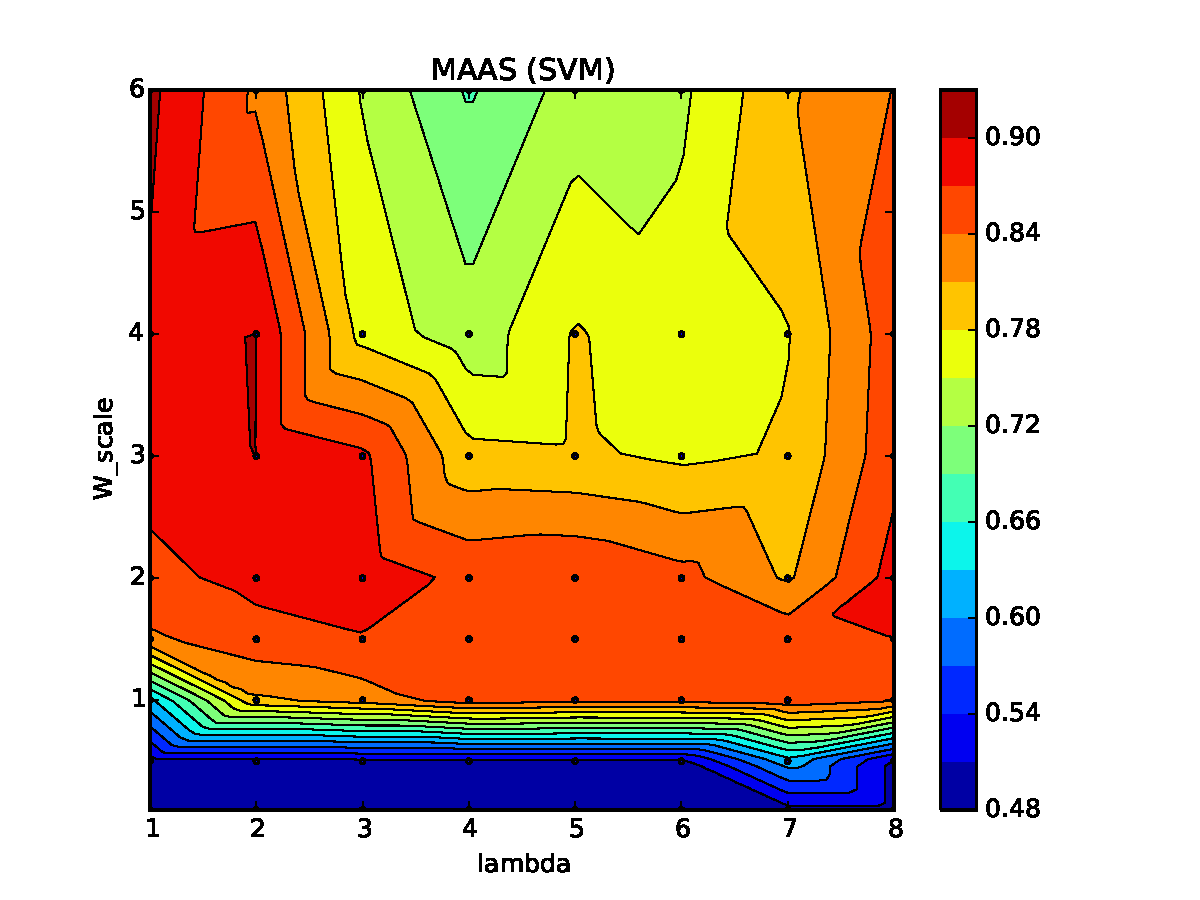
\includegraphics[height=6.0cm]{MAAS_LIQOUT--1_17_30-0_4_5--1_SVM}
	 \label{fig:svm_maas}
}

\subfloat[مدل \lr{SW-A}]{
	 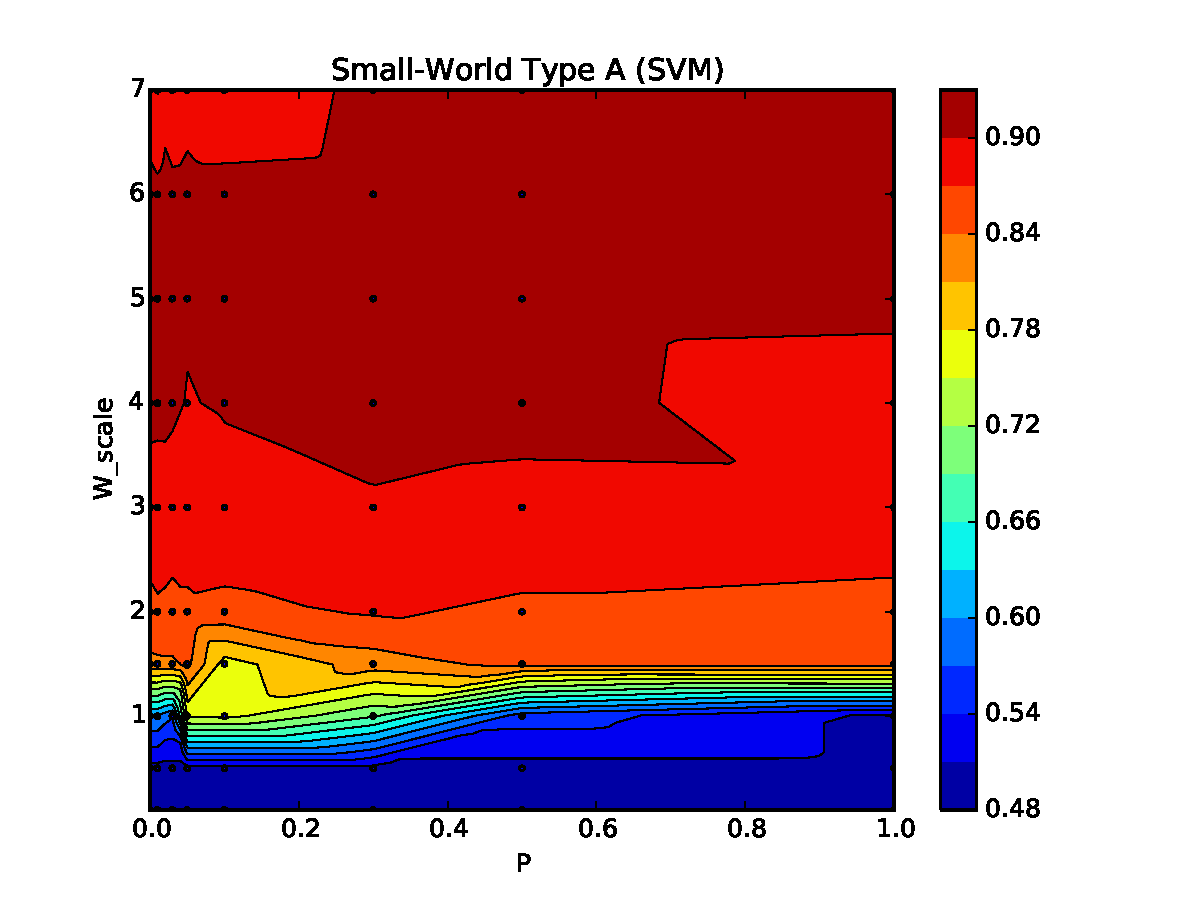
\includegraphics[height=6.0cm]{SW_LIQOUT--1_17_30-0_4_5--A_1_SVM}
	  \label{fig:svm_swa}
}
\subfloat[مدل \lr{SW-B}]{
	 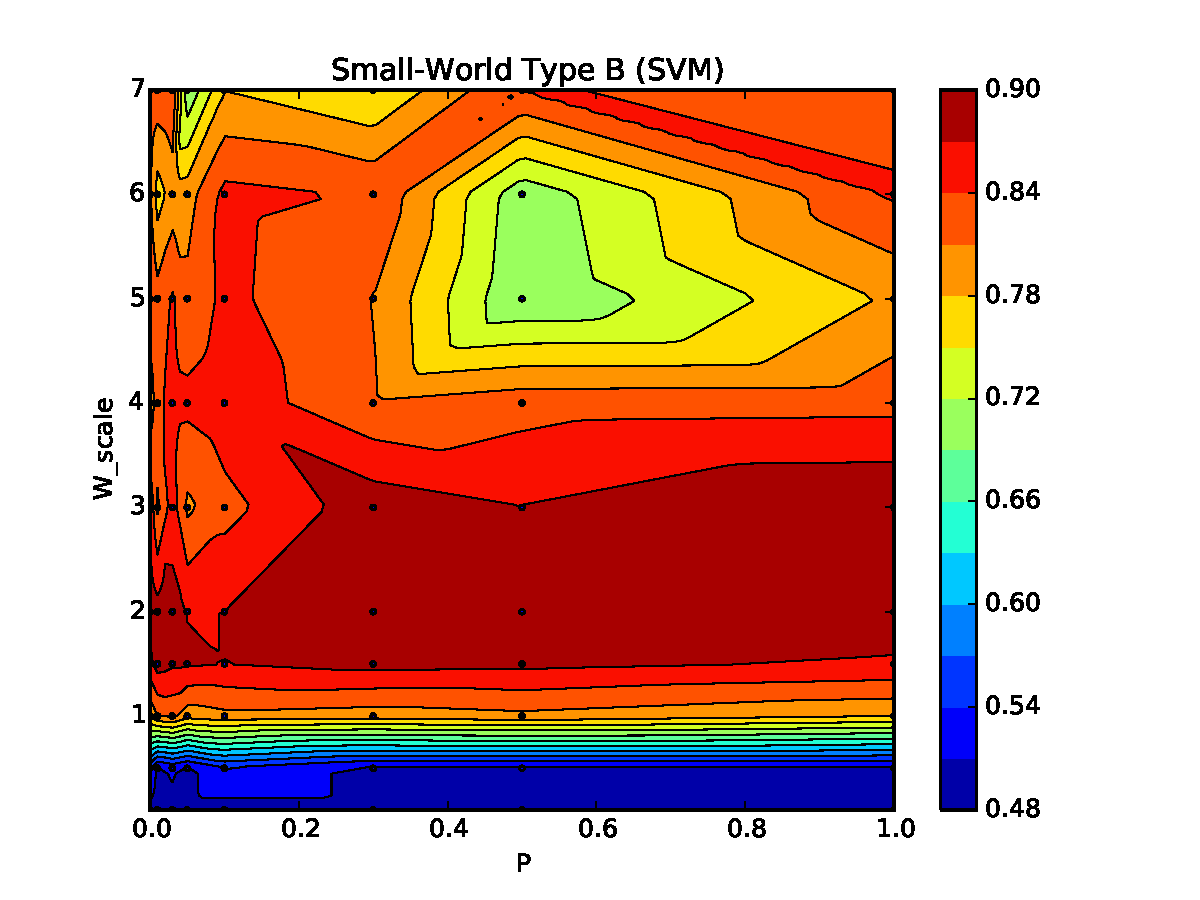
\includegraphics[height=6.0cm]{SW_LIQOUT--1_17_30-0_4_5--B_1_SVM}
	 \label{fig:svm_swb}
}
\caption[عملکرد طبقه‌بند \lr{SVM} برای مدل‌های اتصال]{عملکرد طبقه‌بند \lr{SVM} برای مدل اتصال \subref{fig:svm_maas} \lr{Maas}، \subref{fig:svm_swa} دنیای کوچک نوع \lr{A} و  \subref{fig:svm_swb} دنیای کوچک نوع \lr{B}}
\label{fig:svm}
}
\end{figure}

نواحی به رنگ قرمز در شکل‌های\ref{fig:separation}، \ref{fig:lda} و \ref{fig:svm} نواحی رضایت‌بخش‌تری هستند. در شکل \ref{fig:active} تعداد نورون‌های فعال تحت پارامترهای مختلف نمایش یافته است. نورونی که در کل طول فرآیند حداقل یک بار آتش کرده باشد را نورون «فعال» می‌خوانیم. مشاهده می‌شود که تفکیک‌پذیری یا عملکرد طبقه‌بندی قابل قبول زمانی بدست آمده است که نه خیلی از نورون‌ها فعال بوده و نه تعداد خیلی کمی از آنها فعال شده‌اند. به عبارت دیگر، تعداد خیلی کم یا خیلی زیاد نورون‌های انباره (فیلتر مایع) منجر به عملکرد خوبی نمی‌شود و برای عملکرد قابل قبول، می‌بایست تعداد بینابینی از نورون‌ها فعال شوند. شکل‌های \ref{fig:separation_swa} و \ref{fig:separation_swb} همانطور که انتظار می‌رود نشان می‌دهند که چون در مدل دنیای کوچک مجموع تعداد سیناپس‌ها ثابت می‌ماند، تعداد نورون‌های فعال مشخصا توسط $W_{scale}$  تعیین شده و احتمال سیم‌کشی مجدد $P$ تنها زمانی خود را نشان می‌دهد که ضریب وزن بسیار بزرگ انتخاب شده باشد. 

جدول \ref{res_table} بهترین عملکرد هر مدل اتصال را به ازای همه‌ی مقادیر پارامترهای بررسی شده نشان می‌دهد. همانگونه که مشاهده می‌شود، مدل دنیای کوچک نوع \lr{A} بهترین عملکرد را هم با طبقه‌بند \lr{LDA} و هم با طبقه‌بند \lr{SVM} داشته است. مورد قابل توجه دیگر این است که ترتیب عملکرد خوب این مدل‌ها از پیش توسط معیار تفکیک‌پذیری قابل پیش‌بینی بوده است. هر چند که ماشین‌های حالت مایع بررسی شده، به ازای بهترین پارامتر‌هایشان نتایج به نسبت مشابه با تفاوت قابل اغماض را نتیجه داده‌اند، اما دلیل اصلی انتخاب مدل اتصال دنیای کوچک نوع \lr{A} این است که به ازای گستره‌ی وسیع‌تری از پارامتر‌ها عملکرد قابل‌قبول نشان می‌دهد و از این جهت قابل اطمینان‌تر می‌باشد.

\begin{table}[]
\centering
\caption{بهترین عملکرد مدل‌های اتصال}
\label{res_table}
\begin{tabular}{|l|l|l|l|}
\hline
\textbf{مدل اتصال} & \textbf{معیار تفکیک‌پذیری} & \textbf{LDA} & \textbf{SVM} \\ \hline
\textbf{\lr{Maas}} & $1.34$               & $92.5$        & $91.8$       \\ \hline
\textbf{\lr{SW-A}} & $1.41$               & $92.6$       & $92$         \\ \hline
\textbf{\lr{SW-B}} & $1.36$               & $92.4$       & $91.6$       \\ \hline
\end{tabular}
\end{table}
\subsection{نتیجه‌گیری}
با وجود اینکه بخاطر ساختار غیرخطی و بازگشتی ماشین حالت مایع، تحلیل ریاضیاتی آن بسیار دشوار یا ناممکن است با این حال این امری شناخته شده است که ساختار و به خصوص تعداد سیناپس‌های فیلتر مایع تاثیر بسیاری زیادی بر عملکرد آن دارد و می‌توان با بهره‌وری از یکسری قواعد تجربی به طراحی بهتری از ماشین حالت مایع دست پیدا کرد. در آزمایش‌های صورت گرفته، روش‌های مختلف برقراری اتصال سیناپسی مورد بررسی صورت گرفت و هم از منظر توپولوژی و هم از نظر وزن‌های سیناپسی، مدل‌های اتصال سیناپسی با تراکم و توزیع اتصالات مختلف بررسی شد. ماشین‌های حالت مایع اخیر توجه کاربرد‌های مهندسی را نیز به خود جلب کرده‌اند و ماشین حالت مایع ارائه شده همراه با روش نمایش حالت مایع معرفی شده که بر اساس سازوکار شبکه‌ی سلسله مراتبی، با جلوگیری از افزایش ابعاد مسئله زمانبندی دنباله‌ی ضربه را نیز در نظر می‌گیرد، بر این گرایش صحه می‌گذارد.